\hypertarget{sec-optimization-advanced}{%
\chapter{Advanced Tuning Methods and Black Box Optimization}\label{sec-optimization-advanced}}

\vspace{-15mm}\addtocontents{toc}{\textit{Lennart Schneider and Marc Becker}}

\textbf{Lennart Schneider} \newline 
\emph{Ludwig-Maximilians-Universität München, and Munich Center for
Machine Learning (MCML)}

\textbf{Marc Becker} \newline  \emph{Ludwig-Maximilians-Universität
München, and Munich Center for Machine Learning (MCML)}
\newline \newline 

Having looked at the basic usage of
\href{https://mlr3tuning.mlr-org.com}{\texttt{mlr3tuning}}\index{\texttt{mlr3tuning}},
we will now turn to more advanced methods. We will begin in
Section~\ref{sec-tuning-errors} by continuing to look at
single-objective tuning but will consider what happens when experiments
go wrong and how to prevent fatal errors\index{debugging}. We will then
extend the methodology from Chapter~\ref{sec-optimization} to enable
multi-objective tuning\index{multi-objective tuning}, where learners are
optimized to multiple measures simultaneously, in
Section~\ref{sec-multi-metrics-tuning} we will demonstrate how this is
handled relatively simply in \texttt{mlr3} by making use of the same
classes and methods we have already used. The final two sections focus
on specific optimization methods. Section~\ref{sec-hyperband} looks in
detail at multi-fidelity tuning and the Hyperband tuner, and then
demonstrates it in practice with
\href{https://mlr3hyperband.mlr-org.com}{\texttt{mlr3hyperband}}\index{\texttt{mlr3hyperband}}.
Finally, Section~\ref{sec-bayesian-optimization} takes a deep dive into
black box Bayesian optimization. This is a more theory-heavy section to
motivate the design of the classes and methods in
\href{https://mlr3mbo.mlr-org.com}{\texttt{mlr3mbo}}\index{\texttt{mlr3mbo}}.

\hypertarget{sec-tuning-errors}{%
\section{Error Handling and Memory Management}\label{sec-tuning-errors}}

In this section, we will look at how to use \texttt{mlr3} to ensure that
tuning workflows are efficient and robust. In particular, we will
consider how to enable features that prevent fatal errors leading to
irrecoverable data loss in the middle of an experiment, and then how to
manage tuning experiments that may use up a lot of computer memory.

\hypertarget{sec-encapsulation-fallback}{%
\subsection{Encapsulation and Fallback
Learner}\label{sec-encapsulation-fallback}}

Error handling is discussed in detail in
Section~\ref{sec-error-handling}, however, it is very important in the
context of tuning so here we will just practically demonstrate how to
make use of encapsulation and fallback learners and explain why they are
essential during HPO.

Even in simple machine learning problems, there is a lot of potential
for things to go wrong. For example, when learners do not converge, run
out of memory, or terminate with an error due to issues in the
underlying data. As a common issue, learners can fail if there are
factor levels present in the test data that were not in the training
data, models fail in this case as there have been no
weights/coefficients trained for these new factor levels:

\begin{Shaded}
\begin{Highlighting}[]
\NormalTok{tsk\_pen }\OtherTok{=} \FunctionTok{tsk}\NormalTok{(}\StringTok{"penguins"}\NormalTok{)}
\CommentTok{\# remove rows with missing values}
\NormalTok{tsk\_pen}\SpecialCharTok{$}\FunctionTok{filter}\NormalTok{(tsk\_pen}\SpecialCharTok{$}\NormalTok{row\_ids[}\FunctionTok{complete.cases}\NormalTok{(tsk\_pen}\SpecialCharTok{$}\FunctionTok{data}\NormalTok{())])}
\CommentTok{\# create custom resampling with new factors in test data}
\NormalTok{rsmp\_custom }\OtherTok{=} \FunctionTok{rsmp}\NormalTok{(}\StringTok{"custom"}\NormalTok{)}
\NormalTok{rsmp\_custom}\SpecialCharTok{$}\FunctionTok{instantiate}\NormalTok{(tsk\_pen,}
  \FunctionTok{list}\NormalTok{(tsk\_pen}\SpecialCharTok{$}\NormalTok{row\_ids[tsk\_pen}\SpecialCharTok{$}\FunctionTok{data}\NormalTok{()}\SpecialCharTok{$}\NormalTok{island }\SpecialCharTok{!=} \StringTok{"Torgersen"}\NormalTok{]),}
  \FunctionTok{list}\NormalTok{(tsk\_pen}\SpecialCharTok{$}\NormalTok{row\_ids[tsk\_pen}\SpecialCharTok{$}\FunctionTok{data}\NormalTok{()}\SpecialCharTok{$}\NormalTok{island }\SpecialCharTok{==} \StringTok{"Torgersen"}\NormalTok{])}
\NormalTok{)}
\NormalTok{msr\_ce }\OtherTok{=} \FunctionTok{msr}\NormalTok{(}\StringTok{"classif.ce"}\NormalTok{)}
\NormalTok{tnr\_random }\OtherTok{=} \FunctionTok{tnr}\NormalTok{(}\StringTok{"random\_search"}\NormalTok{)}
\NormalTok{learner }\OtherTok{=} \FunctionTok{lrn}\NormalTok{(}\StringTok{"classif.lda"}\NormalTok{, }\AttributeTok{method =} \StringTok{"t"}\NormalTok{, }\AttributeTok{nu =} \FunctionTok{to\_tune}\NormalTok{(}\DecValTok{3}\NormalTok{, }\DecValTok{10}\NormalTok{))}

\FunctionTok{tune}\NormalTok{(tnr\_random, tsk\_pen, learner, rsmp\_custom, msr\_ce, }\DecValTok{10}\NormalTok{)}
\end{Highlighting}
\end{Shaded}

\begin{verbatim}
Error in lda.default(x, grouping, ...): variable 6 appears to be constant
	within groups
\end{verbatim}

In the above example, we can see the tuning process breaks and we lose
all information about the hyperparameter optimization process. This is
even worse in nested resampling or benchmarking when errors could cause
us to lose all progress across multiple configurations or even learners
and tasks.

Encapsulation\index{encapsulation} (Section~\ref{sec-encapsulation})
allows errors to be isolated and handled, without disrupting the tuning
process. We can tell a learner to encapsulate an error by setting the
\texttt{\$encapsulate} field as follows:

\begin{Shaded}
\begin{Highlighting}[]
\NormalTok{learner}\SpecialCharTok{$}\NormalTok{encapsulate }\OtherTok{=} \FunctionTok{c}\NormalTok{(}\AttributeTok{train =} \StringTok{"evaluate"}\NormalTok{, }\AttributeTok{predict =} \StringTok{"evaluate"}\NormalTok{)}
\end{Highlighting}
\end{Shaded}

Note by passing \texttt{"evaluate"} to both \texttt{train} and
\texttt{predict}, we are telling the learner to set up encapsulation in
both the training and prediction stages (see
Section~\ref{sec-error-handling} for other encapsulation options).

Another common issue that cannot be easily solved during HPO is learners
not converging and the process running indefinitely. We can prevent this
from happening by setting the \texttt{timeout} field in a learner, which
signals the learner to stop if it has been running for that much time
(in seconds), again this can be set for training and prediction
individually:

\begin{Shaded}
\begin{Highlighting}[]
\NormalTok{learner}\SpecialCharTok{$}\NormalTok{timeout }\OtherTok{=} \FunctionTok{c}\NormalTok{(}\AttributeTok{train =} \DecValTok{30}\NormalTok{, }\AttributeTok{predict =} \DecValTok{30}\NormalTok{)}
\end{Highlighting}
\end{Shaded}

Now if either an error occurs, or the model timeout threshold is
reached, then instead of breaking, the learner will simply not make
predictions when errors are found and the result is \texttt{NA} for
resampling iterations with errors. When this happens, our hyperparameter
optimization experiment will fail as we cannot aggregate results across
resampling iterations. Therefore it is essential to select a fallback
learner\index{fallback learner} (Section~\ref{sec-fallback}), which is a
learner that will be fitted if the learner of interest fails.

A common approach is to use a featureless baseline\index{baselines}
(\texttt{lrn("regr.featureless")} or
\texttt{lrn("classif.featureless")}). Below we set
\texttt{lrn("classif.featureless")}, which always predicts the majority
class, by passing this learner to the \texttt{\$fallback} field.

\begin{Shaded}
\begin{Highlighting}[]
\NormalTok{learner}\SpecialCharTok{$}\NormalTok{fallback }\OtherTok{=} \FunctionTok{lrn}\NormalTok{(}\StringTok{"classif.featureless"}\NormalTok{)}
\end{Highlighting}
\end{Shaded}

We can now run our experiment and see errors that occurred during tuning
in the archive.

\begin{Shaded}
\begin{Highlighting}[]
\NormalTok{instance }\OtherTok{=} \FunctionTok{tune}\NormalTok{(tnr\_random, tsk\_pen, learner, rsmp\_custom, msr\_ce,}
  \DecValTok{10}\NormalTok{)}

\FunctionTok{as.data.table}\NormalTok{(instance}\SpecialCharTok{$}\NormalTok{archive)[}\DecValTok{1}\SpecialCharTok{:}\DecValTok{3}\NormalTok{, .(df, classif.ce, errors)]}
\end{Highlighting}
\end{Shaded}

\begin{verbatim}
              df classif.ce errors
1: <function[1]>          1      1
2: <function[1]>          1      1
3: <function[1]>          1      1
\end{verbatim}

\begin{Shaded}
\begin{Highlighting}[]
\CommentTok{\# Reading the error in the first resample result}
\NormalTok{instance}\SpecialCharTok{$}\NormalTok{archive}\SpecialCharTok{$}\FunctionTok{resample\_result}\NormalTok{(}\DecValTok{1}\NormalTok{)}\SpecialCharTok{$}\NormalTok{errors}
\end{Highlighting}
\end{Shaded}

\begin{verbatim}
   iteration                                             msg
1:         1 variable 6 appears to be constant within groups
\end{verbatim}

The learner was tuned without breaking because the errors were
encapsulated and logged before the fallback learners were used for
fitting and predicting:

\begin{Shaded}
\begin{Highlighting}[]
\NormalTok{instance}\SpecialCharTok{$}\NormalTok{result}
\end{Highlighting}
\end{Shaded}

\begin{verbatim}
   nu learner_param_vals  x_domain classif.ce
1:  5          <list[2]> <list[1]>          1
\end{verbatim}

\hypertarget{sec-memory-management}{%
\subsection{Memory Management}\label{sec-memory-management}}

Running a large tuning experiment can use a lot of memory, especially
when using nested resampling. Most of the memory is consumed by the
models since each resampling iteration creates one new model. Storing
the models is therefore disabled by default and in most cases is not
required. The option \texttt{store\_models} in the functions
\href{https://mlr3tuning.mlr-org.com/reference/ti.html}{\texttt{ti()}}
and
\href{https://mlr3tuning.mlr-org.com/reference/auto_tuner.html}{\texttt{auto\_tuner()}}
allows us to enable the storage of the models.

The archive stores a
\href{https://mlr3.mlr-org.com/reference/ResampleResult.html}{\texttt{ResampleResult}}
for each evaluated hyperparameter configuration. The contained
\href{https://mlr3.mlr-org.com/reference/Prediction.html}{\texttt{Prediction}}
objects can also take up a lot of memory, especially with large datasets
and many resampling iterations. We can disable the storage of the
resample results by setting \texttt{store\_benchmark\_result\ =\ FALSE}
in the functions \texttt{ti()} and \texttt{auto\_tuner()}. Note that
without the resample results, it is no longer possible to score the
configurations with another measure.

When we run nested resampling with many outer resampling iterations,
additional memory can be saved if we set
\texttt{store\_tuning\_instance\ =\ FALSE} in the \texttt{auto\_tuner()}
function. However, the functions
\href{https://mlr3tuning.mlr-org.com/reference/extract_inner_tuning_results.html}{\texttt{extract\_inner\_tuning\_results()}}
and
\href{https://mlr3tuning.mlr-org.com/reference/extract_inner_tuning_archives.html}{\texttt{extract\_inner\_tuning\_archives()}}
will then no longer work.

The option \texttt{store\_models\ =\ TRUE} sets
\texttt{store\_benchmark\_result} and \texttt{store\_tuning\_instance}
to \texttt{TRUE} because the models are stored in the benchmark results
which in turn is part of the instance. This also means that
\texttt{store\_benchmark\_result\ =\ TRUE} sets
\texttt{store\_tuning\_instance} to \texttt{TRUE}.

Finally, we can set \texttt{store\_models\ =\ FALSE} in the
\href{https://mlr3.mlr-org.com/reference/resample.html}{\texttt{resample()}}
or
\href{https://mlr3.mlr-org.com/reference/benchmark.html}{\texttt{benchmark()}}
functions to disable the storage of the auto tuners when running nested
resampling. This way we can still access the aggregated performance
(\texttt{rr\$aggregate()}) but lose information about the inner
resampling.

\hypertarget{sec-multi-metrics-tuning}{%
\section{Multi-Objective Tuning}\label{sec-multi-metrics-tuning}}

So far we have considered optimizing a model with respect to one metric,
but multi-criteria, or
multi-objective\index{multi-objective tuning}{\marginnote{\begin{footnotesize}Multi-objective\end{footnotesize}}}
optimization, is also possible. A simple example of multi-objective
optimization might be optimizing a classifier to simultaneously maximize
true positive predictions and minimize false negative predictions. In
another example, consider the single-objective problem of tuning a
neural network\index{neural network} to minimize classification error.
The best-performing model is likely to be quite complex, possibly with
many layers that will have drawbacks like being harder to deploy on
devices with limited resources. In this case, we might want to
simultaneously minimize the classification error and model complexity.

By definition, optimization of multiple metrics means these will be in
competition (otherwise we would only optimize one of them) and therefore
in general no \emph{single} configuration exists that optimizes all
metrics. Therefore, we instead focus on the concept of Pareto
optimality\index{Pareto optimality}. One hyperparameter configuration is
said to \emph{Pareto-dominate} another if the resulting model is equal
or better in all metrics and strictly better in at least one metric. For
example say we are minimizing classification error, CE, and complexity,
CP, for configurations A and B with CE of \(CE_A\) and \(CE_B\)
respectively and CP of \(CP_A\) and \(CP_B\) respectively. Then, A
pareto-dominates B if: 1) \(CE_A \leq CE_B\) and \(CP_A < CP_B\) or; 2)
\(CE_A < CE_B\) and \(CP_A \leq CP_B\). All configurations that are not
Pareto-dominated by any other configuration are called
\emph{Pareto-efficient} and the set of all these configurations is the
\emph{Pareto set}. The metric values corresponding to the Pareto set are
referred to as the Pareto
front\index{Pareto front}{\marginnote{\begin{footnotesize}Pareto
front\end{footnotesize}}}.

The goal of multi-objective hyperparameter optimization is to find a set
of non-dominated solutions so that their corresponding metric values
approximate the Pareto front. We will now demonstrate multi-objective
hyperparameter optimization by tuning a decision tree on
\texttt{tsk("sonar")} with respect to the classification error, as a
measure of model performance, and the number of selected features, as a
measure of model complexity (in a decision tree the number of selected
features is straightforward to obtain by simply counting the number of
unique splitting variables). Methodological details on multi-objective
hyperparameter optimization can be found in Karl et al. (2022) and
Morales-Hernández, Van Nieuwenhuyse, and Rojas Gonzalez (2022).

We will tune \texttt{cp}, \texttt{minsplit}, and \texttt{maxdepth}:

\begin{Shaded}
\begin{Highlighting}[]
\NormalTok{learner }\OtherTok{=} \FunctionTok{lrn}\NormalTok{(}\StringTok{"classif.rpart"}\NormalTok{, }\AttributeTok{cp =} \FunctionTok{to\_tune}\NormalTok{(}\FloatTok{1e{-}04}\NormalTok{, }\FloatTok{1e{-}1}\NormalTok{),}
  \AttributeTok{minsplit =} \FunctionTok{to\_tune}\NormalTok{(}\DecValTok{2}\NormalTok{, }\DecValTok{64}\NormalTok{), }\AttributeTok{maxdepth =} \FunctionTok{to\_tune}\NormalTok{(}\DecValTok{1}\NormalTok{, }\DecValTok{30}\NormalTok{))}

\NormalTok{measures }\OtherTok{=} \FunctionTok{msrs}\NormalTok{(}\FunctionTok{c}\NormalTok{(}\StringTok{"classif.ce"}\NormalTok{, }\StringTok{"selected\_features"}\NormalTok{))}
\end{Highlighting}
\end{Shaded}

As we are tuning with respect to multiple measures, the function
\texttt{ti()} automatically creates a
\href{https://mlr3tuning.mlr-org.com/reference/TuningInstanceMultiCrit.html}{\texttt{TuningInstanceMultiCrit}}
instead of a
\href{https://mlr3tuning.mlr-org.com/reference/TuningInstanceSingleCrit.html}{\texttt{TuningInstanceSingleCrit}}.
Below we set \texttt{store\_models\ =\ TRUE} as this is required by the
selected features measure.

\begin{Shaded}
\begin{Highlighting}[]
\NormalTok{instance }\OtherTok{=} \FunctionTok{ti}\NormalTok{(}
  \AttributeTok{task =} \FunctionTok{tsk}\NormalTok{(}\StringTok{"sonar"}\NormalTok{),}
  \AttributeTok{learner =}\NormalTok{ learner,}
  \AttributeTok{resampling =} \FunctionTok{rsmp}\NormalTok{(}\StringTok{"cv"}\NormalTok{, }\AttributeTok{folds =} \DecValTok{3}\NormalTok{),}
  \AttributeTok{measures =}\NormalTok{ measures,}
  \AttributeTok{terminator =} \FunctionTok{trm}\NormalTok{(}\StringTok{"evals"}\NormalTok{, }\AttributeTok{n\_evals =} \DecValTok{30}\NormalTok{),}
  \AttributeTok{store\_models =} \ConstantTok{TRUE}
\NormalTok{)}
\NormalTok{instance}
\end{Highlighting}
\end{Shaded}

\begin{verbatim}
<TuningInstanceMultiCrit>
* State:  Not optimized
* Objective: <ObjectiveTuning:classif.rpart_on_sonar>
* Search Space:
         id    class lower upper nlevels
1:       cp ParamDbl 1e-04   0.1     Inf
2: minsplit ParamInt 2e+00  64.0      63
3: maxdepth ParamInt 1e+00  30.0      30
* Terminator: <TerminatorEvals>
\end{verbatim}

We can then select and tune a tuning algorithm as usual:

\begin{Shaded}
\begin{Highlighting}[]
\NormalTok{tuner }\OtherTok{=} \FunctionTok{tnr}\NormalTok{(}\StringTok{"random\_search"}\NormalTok{)}
\NormalTok{tuner}\SpecialCharTok{$}\FunctionTok{optimize}\NormalTok{(instance)}
\end{Highlighting}
\end{Shaded}

Finally, we inspect the best-performing configurations, i.e., the Pareto
set, and visualize the corresponding estimated Pareto front
(Figure~\ref{fig-pareto}). Note that the \texttt{selected\_features}
measure is averaged across the folds, so the values in the archive may
not always be integers.

\begin{Shaded}
\begin{Highlighting}[]
\NormalTok{instance}\SpecialCharTok{$}\NormalTok{archive}\SpecialCharTok{$}\FunctionTok{best}\NormalTok{()[, .(cp, minsplit, maxdepth, classif.ce,}
\NormalTok{  selected\_features)]}
\end{Highlighting}
\end{Shaded}

\begin{verbatim}
        cp minsplit maxdepth classif.ce selected_features
1: 0.06881       60        4     0.2596             1.000
2: 0.09451       23       14     0.2596             1.000
3: 0.09891       21       29     0.2596             1.000
4: 0.05475       57       17     0.2596             1.000
5: 0.09774       38       16     0.2596             1.000
6: 0.08944        4        8     0.2547             2.333
\end{verbatim}

\begin{figure}

{\centering 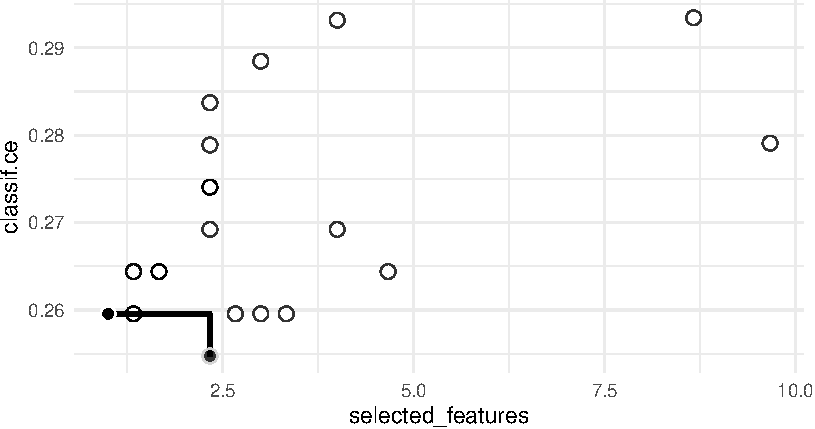
\includegraphics[width=1\textwidth,height=\textheight]{chapters/chapter5/advanced_tuning_methods_and_black_box_optimization_files/figure-pdf/fig-pareto-1.pdf}

}

\caption{\label{fig-pareto}Pareto front of selected features and
classification error. White dots represent tested configurations, each
black dot individually represents a Pareto-optimal configuration and all
black dots together represent the approximated Pareto front.}

\end{figure}

Determining which configuration to deploy from the Pareto front is up to
you. By definition, there is no optimal configuration so this may depend
on your use case, for example, if you would prefer lower complexity at
the cost of higher error then you might prefer a configuration where
\texttt{selected\_features\ =\ 1}.

You can select one configuration and pass it to a learner for training
using \texttt{\$result\_learner\_param\_vals}, so if we want to select
the second configuration we would run:

\begin{Shaded}
\begin{Highlighting}[]
\NormalTok{learner }\OtherTok{=} \FunctionTok{lrn}\NormalTok{(}\StringTok{"classif.rpart"}\NormalTok{)}
\NormalTok{learner}\SpecialCharTok{$}\NormalTok{param\_set}\SpecialCharTok{$}\NormalTok{values }\OtherTok{=}\NormalTok{ instance}\SpecialCharTok{$}\NormalTok{result\_learner\_param\_vals[[}\DecValTok{2}\NormalTok{]]}
\end{Highlighting}
\end{Shaded}

As multi-objective tuning requires manual intervention to select a
configuration, it is currently not possible to use
\href{https://mlr3tuning.mlr-org.com/reference/auto_tuner.html}{\texttt{auto\_tuner()}}.

\hypertarget{sec-hyperband}{%
\section{Multi-Fidelity Tuning via Hyperband}\label{sec-hyperband}}

Increasingly large datasets and search spaces and increasingly complex
models make hyperparameter optimization a time-consuming and
computationally expensive task. To tackle this, some HPO methods make
use of evaluating a configuration at multiple fidelity
levels\index{fidelity}. Multi-fidelity
HPO\index{fidelity!multi-fidelity}{\marginnote{\begin{footnotesize}Multi-fidelity
HPO\end{footnotesize}}} is motivated by the idea that the performance of
a lower-fidelity model is indicative of the full-fidelity model, which
can be used to make HPO more efficient (as we will soon see with
Hyperband).

To unpack what these terms mean and to motivate multi-fidelity tuning,
say that we think a gradient boosting algorithm with up to 1000 rounds
will be a very good fit to our training data. However, we are concerned
this model will take too long to tune and train. Therefore, we want to
gauge the performance of this model using a similar model that is
quicker to train by setting a smaller number of rounds. In this example,
the hyperparameter controlling the number of rounds is a \emph{fidelity
parameter}, as it controls the tradeoff between model performance and
speed. The different configurations of this parameter are known as
\emph{fidelity levels}. We refer to the model with 1000 rounds as the
model at \emph{full-fidelity} and we want to approximate this model's
performance using models at different fidelity levels. Lower fidelity
levels result in low-fidelity models that are quicker to train but may
poorly predict the full-fidelity model's performance. On the other hand,
higher fidelity levels result in high-fidelity models that are slower to
train but may better indicate the full-fidelity model's performance.

Other common models that have natural fidelity parameters include neural
networks\index{neural network} (number of epochs) and random
forests\index{random forest} (number of trees). The proportion of data
to subsample before running any algorithm can also be viewed as a
model-agnostic fidelity parameter, we will return to this in
Section~\ref{sec-hyperband-example-svm}.

\hypertarget{hyperband-and-successive-halving}{%
\subsection{Hyperband and Successive
Halving}\label{hyperband-and-successive-halving}}

A popular multi-fidelity HPO algorithm is \emph{Hyperband} (Li et al.
2018). After having evaluated randomly sampled configurations on low
fidelities, Hyperband\index{hyperband} iteratively allocates more
resources to promising configurations and terminates low-performing ones
early. Hyperband builds upon the Successive Halving algorithm by
Jamieson and Talwalkar (2016). Successive Halving is initialized with a
number of starting configurations \(m_0\), the proportion of
configurations discarded in each stage \(\eta\), and the minimum,
\(r{_{0}}\), and maximum, \(r{_{max}}\), budget (fidelity) of a single
evaluation. The algorithm starts by sampling \(m_0\) random
configurations and allocating the minimum budget \(r{_{0}}\) to them.
The configurations are evaluated and \(\frac{\eta - 1}{\eta}\) of the
worst-performing configurations are discarded. The remaining
configurations are promoted to the next stage, or `bracket', and
evaluated on a larger budget. This continues until one or more
configurations are evaluated on the maximum budget \(r{_{max}}\) and the
best-performing configuration is selected. The total number of stages is
calculated so that each stage consumes approximately the same overall
budget. A big disadvantage of this method is that it is unclear if it is
better to start with many configurations (large \(m_0\)) and a small
budget or fewer configurations (small \(m_0\)) but a larger budget.

Hyperband solves this problem by running Successive Halving with
different numbers of starting configurations, each at different budget
levels \(r_{0}\). The algorithm is initialized with the same \(\eta\)
and \(r_{max}\) parameters (but not \(m_0\)). Each bracket starts with a
different budget, \(r_0\), where smaller values mean that more
configurations can be evaluated and so the most exploratory bracket
(i.e., the one with the most number of stages) is allocated the global
minimum budget \(r_{min}\). In each bracket, the starting budget
increases by a factor of \(\eta\) until the last bracket essentially
performs a random search with the full budget \(r_{max}\). The total
number of brackets, \(s_{max} + 1\), is calculated as
\(s_{max} = {\log_\eta \frac{r_{max}}{r_{min}}}\). The number of
starting configurations \(m_0\) of each bracket are calculated so that
each bracket uses approximately the same amount of budget. The optimal
hyperparameter configuration in each bracket is the configuration with
the best performance in the final stage. The optimal hyperparameter
configuration at the end of tuning is the configuration with the best
performance across all brackets.

An example Hyperband schedule is given in Table~\ref{tbl-hyperband}
where \(s = 3\) is the most exploratory bracket and \(s = 0\)
essentially performs a random search using the full budget.
Table~\ref{tbl-hyperband-eg} demonstrates how this schedule may look if
we were to tune 20 different hyperparameter configurations; note that
each entry in the table is a unique ID referring to a possible
configuration of multiple hyperparameters to tune.

\hypertarget{tbl-hyperband}{}
\begin{longtable}[]{@{}
  >{\raggedright\arraybackslash}p{(\columnwidth - 16\tabcolsep) * \real{0.0645}}
  >{\raggedright\arraybackslash}p{(\columnwidth - 16\tabcolsep) * \real{0.1075}}
  >{\raggedright\arraybackslash}p{(\columnwidth - 16\tabcolsep) * \real{0.1075}}
  >{\raggedright\arraybackslash}p{(\columnwidth - 16\tabcolsep) * \real{0.1075}}
  >{\raggedright\arraybackslash}p{(\columnwidth - 16\tabcolsep) * \real{0.1075}}
  >{\raggedright\arraybackslash}p{(\columnwidth - 16\tabcolsep) * \real{0.1075}}
  >{\raggedright\arraybackslash}p{(\columnwidth - 16\tabcolsep) * \real{0.1075}}
  >{\raggedright\arraybackslash}p{(\columnwidth - 16\tabcolsep) * \real{0.1075}}
  >{\raggedright\arraybackslash}p{(\columnwidth - 16\tabcolsep) * \real{0.1075}}@{}}
\caption{\label{tbl-hyperband}Hyperband schedule with the number of
configurations, \(m_{i}\), and resources, \(r_{i}\), for each bracket,
\(s\), and stage, \(i\), when \(\eta = 2\), \(r{_{min}} = 1\) and
\(r{_{max}} = 8\).}\tabularnewline
\toprule\noalign{}
\begin{minipage}[b]{\linewidth}\raggedright
\end{minipage} &
\multicolumn{2}{>{\raggedright\arraybackslash}p{(\columnwidth - 16\tabcolsep) * \real{0.2151} + 2\tabcolsep}}{%
\begin{minipage}[b]{\linewidth}\raggedright
\(s = 3\)
\end{minipage}} &
\multicolumn{2}{>{\raggedright\arraybackslash}p{(\columnwidth - 16\tabcolsep) * \real{0.2151} + 2\tabcolsep}}{%
\begin{minipage}[b]{\linewidth}\raggedright
\(s = 2\)
\end{minipage}} &
\multicolumn{2}{>{\raggedright\arraybackslash}p{(\columnwidth - 16\tabcolsep) * \real{0.2151} + 2\tabcolsep}}{%
\begin{minipage}[b]{\linewidth}\raggedright
\(s = 1\)
\end{minipage}} &
\multicolumn{2}{>{\raggedright\arraybackslash}p{(\columnwidth - 16\tabcolsep) * \real{0.2151} + 2\tabcolsep}@{}}{%
\begin{minipage}[b]{\linewidth}\raggedright
\(s = 0\)
\end{minipage}} \\
\begin{minipage}[b]{\linewidth}\raggedright
\(i\)
\end{minipage} & \begin{minipage}[b]{\linewidth}\raggedright
\(m_{i}\)
\end{minipage} & \begin{minipage}[b]{\linewidth}\raggedright
\(r_{i}\)
\end{minipage} & \begin{minipage}[b]{\linewidth}\raggedright
\(m_{i}\)
\end{minipage} & \begin{minipage}[b]{\linewidth}\raggedright
\(r_{i}\)
\end{minipage} & \begin{minipage}[b]{\linewidth}\raggedright
\(m_{i}\)
\end{minipage} & \begin{minipage}[b]{\linewidth}\raggedright
\(r_{i}\)
\end{minipage} & \begin{minipage}[b]{\linewidth}\raggedright
\(m_{i}\)
\end{minipage} & \begin{minipage}[b]{\linewidth}\raggedright
\(r_{i}\)
\end{minipage} \\
\midrule\noalign{}
\endfirsthead
\toprule\noalign{}
\begin{minipage}[b]{\linewidth}\raggedright
\end{minipage} &
\multicolumn{2}{>{\raggedright\arraybackslash}p{(\columnwidth - 16\tabcolsep) * \real{0.2151} + 2\tabcolsep}}{%
\begin{minipage}[b]{\linewidth}\raggedright
\(s = 3\)
\end{minipage}} &
\multicolumn{2}{>{\raggedright\arraybackslash}p{(\columnwidth - 16\tabcolsep) * \real{0.2151} + 2\tabcolsep}}{%
\begin{minipage}[b]{\linewidth}\raggedright
\(s = 2\)
\end{minipage}} &
\multicolumn{2}{>{\raggedright\arraybackslash}p{(\columnwidth - 16\tabcolsep) * \real{0.2151} + 2\tabcolsep}}{%
\begin{minipage}[b]{\linewidth}\raggedright
\(s = 1\)
\end{minipage}} &
\multicolumn{2}{>{\raggedright\arraybackslash}p{(\columnwidth - 16\tabcolsep) * \real{0.2151} + 2\tabcolsep}@{}}{%
\begin{minipage}[b]{\linewidth}\raggedright
\(s = 0\)
\end{minipage}} \\
\begin{minipage}[b]{\linewidth}\raggedright
\(i\)
\end{minipage} & \begin{minipage}[b]{\linewidth}\raggedright
\(m_{i}\)
\end{minipage} & \begin{minipage}[b]{\linewidth}\raggedright
\(r_{i}\)
\end{minipage} & \begin{minipage}[b]{\linewidth}\raggedright
\(m_{i}\)
\end{minipage} & \begin{minipage}[b]{\linewidth}\raggedright
\(r_{i}\)
\end{minipage} & \begin{minipage}[b]{\linewidth}\raggedright
\(m_{i}\)
\end{minipage} & \begin{minipage}[b]{\linewidth}\raggedright
\(r_{i}\)
\end{minipage} & \begin{minipage}[b]{\linewidth}\raggedright
\(m_{i}\)
\end{minipage} & \begin{minipage}[b]{\linewidth}\raggedright
\(r_{i}\)
\end{minipage} \\
\midrule\noalign{}
\endhead
\bottomrule\noalign{}
\endlastfoot
0 & 8 & 1 & 6 & 2 & 4 & 4 & 4 & 8 \\
1 & 4 & 2 & 3 & 4 & 2 & 8 & & \\
2 & 2 & 4 & 1 & 8 & & & & \\
3 & 1 & 8 & & & & & & \\
\end{longtable}

\hypertarget{tbl-hyperband-eg}{}
\begin{longtable}[]{@{}
  >{\raggedright\arraybackslash}p{(\columnwidth - 8\tabcolsep) * \real{0.0588}}
  >{\raggedright\arraybackslash}p{(\columnwidth - 8\tabcolsep) * \real{0.2353}}
  >{\raggedright\arraybackslash}p{(\columnwidth - 8\tabcolsep) * \real{0.2353}}
  >{\raggedright\arraybackslash}p{(\columnwidth - 8\tabcolsep) * \real{0.2353}}
  >{\raggedright\arraybackslash}p{(\columnwidth - 8\tabcolsep) * \real{0.2353}}@{}}
\caption{\label{tbl-hyperband-eg}Hyperparameter configurations in each
stage and bracket from the schedule in Table~\ref{tbl-hyperband}.
Entries are unique identifiers for tested hyperparameter configurations
(HPCs). \(HPC^*_s\) is the optimal hyperparameter configuration in
bracket \(s\) and \(HPC^*\) is the optimal hyperparameter configuration
across all brackets.}\tabularnewline
\toprule\noalign{}
\begin{minipage}[b]{\linewidth}\raggedright
\end{minipage} & \begin{minipage}[b]{\linewidth}\raggedright
\(s = 3\)
\end{minipage} & \begin{minipage}[b]{\linewidth}\raggedright
\(s = 2\)
\end{minipage} & \begin{minipage}[b]{\linewidth}\raggedright
\(s = 1\)
\end{minipage} & \begin{minipage}[b]{\linewidth}\raggedright
\(s = 0\)
\end{minipage} \\
\midrule\noalign{}
\endfirsthead
\toprule\noalign{}
\begin{minipage}[b]{\linewidth}\raggedright
\end{minipage} & \begin{minipage}[b]{\linewidth}\raggedright
\(s = 3\)
\end{minipage} & \begin{minipage}[b]{\linewidth}\raggedright
\(s = 2\)
\end{minipage} & \begin{minipage}[b]{\linewidth}\raggedright
\(s = 1\)
\end{minipage} & \begin{minipage}[b]{\linewidth}\raggedright
\(s = 0\)
\end{minipage} \\
\midrule\noalign{}
\endhead
\bottomrule\noalign{}
\endlastfoot
\(i = 0\) & \(\{1, 2, 3, 4, 5, 6, 7, 8\}\) &
\(\{9, 10, 11, 12, 13, 14\}\) & \(\{15, 16, 17, 18\}\) &
\(\{19, 20, 21, 22\}\) \\
\(i = 1\) & \(\{1, 2, 7, 8\}\) & \(\{9, 14, 15\}\) & \(\{20, 21\}\) & \\
\(i = 2\) & \(\{1, 8\}\) & \(\{15\}\) & & \\
\(i = 3\) & \(\{1\}\) & & & \\
\(HPC^*_s\) & \(\{1\}\) & \(\{15\}\) & \(\{21\}\) & \(\{22\}\) \\
\(HPC^*\) & \(\{15\}\) & & & \\
\end{longtable}

\hypertarget{mlr3hyperband}{%
\subsection{mlr3hyperband}\label{mlr3hyperband}}

The Successive Halving and Hyperband algorithms are implemented in
\href{https://mlr3hyperband.mlr-org.com}{\texttt{mlr3hyperband}}\index{\texttt{mlr3hyperband}}
as \texttt{tnr("successive\_halving")} and \texttt{tnr("hyperband")}
respectively; in this section, we will only showcase the Hyperband
method.

By example, we will optimize \texttt{lrn("classif.xgboost")} on
\texttt{tsk("sonar")} and use the number of boosting iterations
(\texttt{nrounds}) as the fidelity parameter, this is a suitable choice
as increasing iterations increases model training time but generally
also improves performance. Hyperband will allocate increasingly more
boosting iterations to well-performing hyperparameter configurations.

We will load the learner and define the search space. We specify a range
from 16 (\(r_{min}\)) to 128 (\(r_{max}\)) boosting iterations and tag
the parameter with \texttt{"budget"} to identify it as a fidelity
parameter. For the other hyperparameters, we take the search space for
XGBoost from Bischl et al. (2023), which usually works well for a wide
range of datasets.

\begin{Shaded}
\begin{Highlighting}[]
\FunctionTok{library}\NormalTok{(mlr3hyperband)}

\NormalTok{learner }\OtherTok{=} \FunctionTok{lrn}\NormalTok{(}\StringTok{"classif.xgboost"}\NormalTok{)}
\NormalTok{learner}\SpecialCharTok{$}\NormalTok{param\_set}\SpecialCharTok{$}\FunctionTok{set\_values}\NormalTok{(}
  \AttributeTok{nrounds           =} \FunctionTok{to\_tune}\NormalTok{(}\FunctionTok{p\_int}\NormalTok{(}\DecValTok{16}\NormalTok{, }\DecValTok{128}\NormalTok{, }\AttributeTok{tags =} \StringTok{"budget"}\NormalTok{)),}
  \AttributeTok{eta               =} \FunctionTok{to\_tune}\NormalTok{(}\FloatTok{1e{-}4}\NormalTok{, }\DecValTok{1}\NormalTok{, }\AttributeTok{logscale =} \ConstantTok{TRUE}\NormalTok{),}
  \AttributeTok{max\_depth         =} \FunctionTok{to\_tune}\NormalTok{(}\DecValTok{1}\NormalTok{, }\DecValTok{20}\NormalTok{),}
  \AttributeTok{colsample\_bytree  =} \FunctionTok{to\_tune}\NormalTok{(}\FloatTok{1e{-}1}\NormalTok{, }\DecValTok{1}\NormalTok{),}
  \AttributeTok{colsample\_bylevel =} \FunctionTok{to\_tune}\NormalTok{(}\FloatTok{1e{-}1}\NormalTok{, }\DecValTok{1}\NormalTok{),}
  \AttributeTok{lambda            =} \FunctionTok{to\_tune}\NormalTok{(}\FloatTok{1e{-}3}\NormalTok{, }\FloatTok{1e3}\NormalTok{, }\AttributeTok{logscale =} \ConstantTok{TRUE}\NormalTok{),}
  \AttributeTok{alpha             =} \FunctionTok{to\_tune}\NormalTok{(}\FloatTok{1e{-}3}\NormalTok{, }\FloatTok{1e3}\NormalTok{, }\AttributeTok{logscale =} \ConstantTok{TRUE}\NormalTok{),}
  \AttributeTok{subsample         =} \FunctionTok{to\_tune}\NormalTok{(}\FloatTok{1e{-}1}\NormalTok{, }\DecValTok{1}\NormalTok{)}
\NormalTok{)}
\end{Highlighting}
\end{Shaded}

We now construct the tuning instance and a hyperband tuner with
\texttt{eta\ =\ 2}. We use \texttt{trm("none")} and set the
\texttt{repetitions} control parameter to \texttt{1} so that Hyperband
can terminate itself after all brackets have been evaluated a single
time. Note that setting \texttt{repetition\ =\ Inf} can be useful if you
want a terminator to stop the optimization, for example, based on
runtime. The
\href{https://mlr3hyperband.mlr-org.com/reference/hyperband_schedule.html}{\texttt{hyperband\_schedule()}}
function can be used to display the schedule across the given fidelity
levels and budget increase factor.

\begin{Shaded}
\begin{Highlighting}[]
\NormalTok{instance }\OtherTok{=} \FunctionTok{ti}\NormalTok{(}
  \AttributeTok{task =} \FunctionTok{tsk}\NormalTok{(}\StringTok{"sonar"}\NormalTok{),}
  \AttributeTok{learner =}\NormalTok{ learner,}
  \AttributeTok{resampling =} \FunctionTok{rsmp}\NormalTok{(}\StringTok{"holdout"}\NormalTok{),}
  \AttributeTok{measures =} \FunctionTok{msr}\NormalTok{(}\StringTok{"classif.ce"}\NormalTok{),}
  \AttributeTok{terminator =} \FunctionTok{trm}\NormalTok{(}\StringTok{"none"}\NormalTok{)}
\NormalTok{)}

\NormalTok{tuner }\OtherTok{=} \FunctionTok{tnr}\NormalTok{(}\StringTok{"hyperband"}\NormalTok{, }\AttributeTok{eta =} \DecValTok{2}\NormalTok{, }\AttributeTok{repetitions =} \DecValTok{1}\NormalTok{)}

\FunctionTok{hyperband\_schedule}\NormalTok{(}\AttributeTok{r\_min =} \DecValTok{16}\NormalTok{, }\AttributeTok{r\_max =} \DecValTok{128}\NormalTok{, }\AttributeTok{eta =} \DecValTok{2}\NormalTok{)}
\end{Highlighting}
\end{Shaded}

\begin{verbatim}
    bracket stage budget n
 1:       3     0     16 8
 2:       3     1     32 4
 3:       3     2     64 2
 4:       3     3    128 1
 5:       2     0     32 6
 6:       2     1     64 3
 7:       2     2    128 1
 8:       1     0     64 4
 9:       1     1    128 2
10:       0     0    128 4
\end{verbatim}

Finally, we can tune as normal and print the result and archive. Note
that the archive resulting from a Hyperband run contains the additional
columns \texttt{bracket} and \texttt{stage} which break down the results
by the corresponding bracket and stage.

\begin{Shaded}
\begin{Highlighting}[]
\NormalTok{tuner}\SpecialCharTok{$}\FunctionTok{optimize}\NormalTok{(instance)}
\end{Highlighting}
\end{Shaded}

\begin{verbatim}
   nrounds    eta max_depth colsample_bytree colsample_bylevel lambda
1:      64 -2.618         3            0.666            0.4722 -5.816
5 variables not shown: [alpha, subsample, learner_param_vals, x_domain, classif.ce]
\end{verbatim}

\begin{Shaded}
\begin{Highlighting}[]
\NormalTok{instance}\SpecialCharTok{$}\NormalTok{result[, .(classif.ce, nrounds)]}
\end{Highlighting}
\end{Shaded}

\begin{verbatim}
   classif.ce nrounds
1:     0.1304      64
\end{verbatim}

\begin{Shaded}
\begin{Highlighting}[]
\FunctionTok{as.data.table}\NormalTok{(instance}\SpecialCharTok{$}\NormalTok{archive)[,}
\NormalTok{  .(bracket, stage, classif.ce, eta, max\_depth, colsample\_bytree)]}
\end{Highlighting}
\end{Shaded}

\begin{verbatim}
    bracket stage classif.ce    eta max_depth colsample_bytree
 1:       3     0     0.4203 -6.664         8           0.8640
 2:       3     0     0.5942 -3.139         2           0.8902
 3:       3     0     0.2899 -6.968        15           0.8204
 4:       3     0     0.2609 -6.555        12           0.6761
 5:       3     0     0.2174 -2.618         3           0.6660
---                                                           
31:       0     0     0.2609 -8.070         1           0.9717
32:       3     3     0.1594 -2.618         3           0.6660
33:       2     2     0.1739 -6.455         5           0.9380
34:       1     1     0.2029 -4.509        10           0.7219
35:       1     1     0.2464 -5.749         3           0.2345
\end{verbatim}

\hypertarget{sec-bayesian-optimization}{%
\section{Bayesian Optimization}\label{sec-bayesian-optimization}}

In this section, we will take a deep dive into Bayesian
optimization\index{Bayesian optimization} (BO), also known as Model
Based Optimization
(MBO)\index{model based optimization|see{Bayesian optimization}}. The
design of BO is more complex than what we have seen so far in other
tuning methods so to help motivate this we will spend a little more time
in this section on theory and methodology.

In hyperparameter optimization\index{hyperparameter optimization}
(Chapter~\ref{sec-optimization}), learners are passed a hyperparameter
configuration and evaluated on a given task via a resampling technique
to estimate its generalization performance with the goal to find the
optimal hyperparameter configuration. In general, no analytical
description for the mapping from hyperparameter configuration to
performance exists and gradient information is also not available. HPO
is, therefore, a prime example for black box
optimization\index{black box optimization}{\marginnote{\begin{footnotesize}Black
Box Optimization\end{footnotesize}}}, which considers the optimization
of a function whose mathematical structure and analytical description is
unknown or unexploitable. As a result, the only observable information
is the output value (i.e., generalization performance) of the function
given an input value (i.e., hyperparameter configuration). In fact, as
evaluating the performance of a learner can take a substantial amount of
time, HPO is quite an expensive black box optimization problem. Black
box optimization problems occur in the real-world, for example they are
encountered quite often in engineering such as in modeling experiments
like crash tests or chemical reactions.

Many optimization algorithm classes exist that can be used for black box
optimization, which differ in how they tackle this problem; for example
we saw in Chapter~\ref{sec-optimization} methods including grid/random
search and briefly discussed evolutionary strategies. Bayesian
optimization refers to a class of sample-efficient iterative global
black box optimization algorithms that rely on a `surrogate model'
trained on observed data to model the black box function. This surrogate
model is typically a non-linear regression model that tries to capture
the unknown function using limited observed data. During each iteration,
BO algorithms employ an `acquisition function' to determine the next
candidate point for evaluation. This function measures the expected
`utility' of each point within the search space based on the prediction
of the surrogate model. The algorithm then selects the candidate point
with the best acquisition function value and evaluates the black box
function at that point to then update the surrogate model. This
iterative process continues until a termination criterion is met, such
as reaching a pre-specified maximum number of evaluations or achieving a
desired level of performance. BO is a powerful method that often results
in good optimization performance, especially if the cost of the black
box evaluation becomes expensive and the optimization budget is tight.

In the rest of this section, we will first provide an introduction to
black box optimization with the
\href{https://bbotk.mlr-org.com}{\texttt{bbotk}}\index{\texttt{bbotk}}
package and then introduce the building blocks of BO algorithms and
examine their interplay and interaction during the optimization process
before we assemble these building blocks in a ready to use black box
optimizer with
\href{https://mlr3mbo.mlr-org.com}{\texttt{mlr3mbo}}\index{\texttt{mlr3mbo}}.
Readers who are primarily interested in how to utilize BO for HPO
without delving deep into the underlying building blocks may want to
skip to Section~\ref{sec-bayesian-tuning}. Detailed introductions to
black box optimization and BO are given in Bischl et al. (2023), Feurer
and Hutter (2019) and Garnett (2022).

As a running example throughout this section, we will optimize the
sinusoidal function
\(f: [0, 1] \rightarrow \mathbb{R}, x \mapsto 2x + \sin(14x)\)
(Figure~\ref{fig-bayesian-optimization-sinusoidal}), which is
characterized by two local minima and one global minimum.

\hypertarget{sec-black-box-optimization}{%
\subsection{Black Box Optimization}\label{sec-black-box-optimization}}

The
\href{https://bbotk.mlr-org.com}{\texttt{bbotk}}\index{\texttt{bbotk}}
(black box optimization toolkit) package is the workhorse package for
general black box optimization within the \texttt{mlr3} ecosystem. At
the heart of the package are the R6 classes:

\begin{itemize}
\tightlist
\item
  \href{https://bbotk.mlr-org.com/reference/OptimInstanceSingleCrit.html}{\texttt{OptimInstanceSingleCrit}}
  and
  \href{https://bbotk.mlr-org.com/reference/OptimInstanceMultiCrit.html}{\texttt{OptimInstanceMultiCrit}},
  which are used to construct an optimization
  instance\index{optimization instance}{\marginnote{\begin{footnotesize}Optimization
  Instance\end{footnotesize}}} that describes the optimization problem
  and stores the results
\item
  \href{https://bbotk.mlr-org.com/reference/Optimizer.html}{\texttt{Optimizer}}
  which is used to construct and configure optimization algorithms.
\end{itemize}

These classes might look familiar after reading
Chapter~\ref{sec-optimization}, and in fact
\href{https://mlr3tuning.mlr-org.com/reference/TuningInstanceSingleCrit.html}{\texttt{TuningInstanceSingleCrit}}
and
\href{https://mlr3tuning.mlr-org.com/reference/TuningInstanceMultiCrit.html}{\texttt{TuningInstanceMultiCrit}}
inherit from \texttt{OptimInstanceSingle/MultiCrit} and
\href{https://mlr3tuning.mlr-org.com/reference/Tuner.html}{\texttt{Tuner}}
is closely based on \texttt{Optimizer}.

\texttt{OptimInstanceSingleCrit} relies on an
\href{https://bbotk.mlr-org.com/reference/Objective.html}{\texttt{Objective}}\index{\texttt{Objective}}{\marginnote{\begin{footnotesize}\texttt{Objective}\end{footnotesize}}}
function that wraps the actual mapping from a domain (all possible
function inputs) to a codomain (all possible function outputs).

Objective functions can be created using different classes, all of which
inherit from
\href{https://bbotk.mlr-org.com/reference/Objective.html}{\texttt{Objective}}.
These classes provide different ways to define and evaluate objective
functions and picking the right one will reduce type conversion
overhead:

\begin{itemize}
\tightlist
\item
  \href{https://bbotk.mlr-org.com/reference/ObjectiveRFun.html}{\texttt{ObjectiveRFun}}
  wraps a function that takes a list describing a \emph{single
  configuration} as input where elements can be of any type. It is
  suitable when the underlying function evaluation mechanism is given by
  evaluating a single configuration at a time.
\item
  \href{https://bbotk.mlr-org.com/reference/ObjectiveRFunMany.html}{\texttt{ObjectiveRFunMany}}
  wraps a function that takes a list of \emph{multiple configurations}
  as input where elements can be of any type and even mixed types. It is
  useful when the function evaluation of multiple configurations can be
  parallelized.
\item
  \href{https://bbotk.mlr-org.com/reference/ObjectiveRFunDt.html}{\texttt{ObjectiveRFunDt}}
  wraps a function that operates on a \texttt{data.table}. It allows for
  efficient vectorized or batched evaluations directly on the
  \texttt{data.table} object, avoiding unnecessary data type
  conversions.
\end{itemize}

To start translating our problem to code we will use the
\href{https://bbotk.mlr-org.com/reference/ObjectiveRFun.html}{\texttt{ObjectiveRFun}}
class to take a single configuration as input. The \texttt{Objective}
requires specification of the function to optimize its domain and
codomain. By tagging the codomain with \texttt{"minimize"} or
\texttt{"maximize"} we specify the optimization direction. Note how
below our optimization function takes a \texttt{list} as an input with
one element called \texttt{x}.

\begin{Shaded}
\begin{Highlighting}[]
\FunctionTok{library}\NormalTok{(bbotk)}
\NormalTok{sinus\_1D }\OtherTok{=} \ControlFlowTok{function}\NormalTok{(xs) }\DecValTok{2} \SpecialCharTok{*}\NormalTok{ xs}\SpecialCharTok{$}\NormalTok{x }\SpecialCharTok{*} \FunctionTok{sin}\NormalTok{(}\DecValTok{14} \SpecialCharTok{*}\NormalTok{ xs}\SpecialCharTok{$}\NormalTok{x)}

\NormalTok{domain }\OtherTok{=} \FunctionTok{ps}\NormalTok{(}\AttributeTok{x =} \FunctionTok{p\_dbl}\NormalTok{(}\AttributeTok{lower =} \DecValTok{0}\NormalTok{, }\AttributeTok{upper =} \DecValTok{1}\NormalTok{))}
\NormalTok{codomain }\OtherTok{=} \FunctionTok{ps}\NormalTok{(}\AttributeTok{y =} \FunctionTok{p\_dbl}\NormalTok{(}\AttributeTok{tags =} \StringTok{"minimize"}\NormalTok{))}
\NormalTok{objective }\OtherTok{=}\NormalTok{ ObjectiveRFun}\SpecialCharTok{$}\FunctionTok{new}\NormalTok{(sinus\_1D,}
  \AttributeTok{domain =}\NormalTok{ domain, }\AttributeTok{codomain =}\NormalTok{ codomain)}
\end{Highlighting}
\end{Shaded}

We can visualize our objective by generating a grid of points on which
we evaluate the function
(Figure~\ref{fig-bayesian-optimization-sinusoidal}), this will help us
identify its local minima and global minimum.

\begin{Shaded}
\begin{Highlighting}[]
\FunctionTok{library}\NormalTok{(ggplot2)}

\NormalTok{xydt }\OtherTok{=} \FunctionTok{generate\_design\_grid}\NormalTok{(domain, }\AttributeTok{resolution =} \DecValTok{1001}\NormalTok{)}\SpecialCharTok{$}\NormalTok{data}
\NormalTok{xydt[, y }\SpecialCharTok{:}\ErrorTok{=}\NormalTok{ objective}\SpecialCharTok{$}\FunctionTok{eval\_dt}\NormalTok{(xydt)}\SpecialCharTok{$}\NormalTok{y]}
\NormalTok{optima }\OtherTok{=} \FunctionTok{data.table}\NormalTok{(}\AttributeTok{x =} \FunctionTok{c}\NormalTok{(}\DecValTok{0}\NormalTok{, }\FloatTok{0.3509406}\NormalTok{, }\FloatTok{0.7918238}\NormalTok{))}
\NormalTok{optima[, y }\SpecialCharTok{:}\ErrorTok{=}\NormalTok{ objective}\SpecialCharTok{$}\FunctionTok{eval\_dt}\NormalTok{(optima)}\SpecialCharTok{$}\NormalTok{y]}
\NormalTok{optima[, type }\SpecialCharTok{:}\ErrorTok{=} \FunctionTok{c}\NormalTok{(}\StringTok{"local"}\NormalTok{, }\StringTok{"local"}\NormalTok{, }\StringTok{"global"}\NormalTok{)]}

\FunctionTok{ggplot}\NormalTok{(}\FunctionTok{aes}\NormalTok{(}\AttributeTok{x =}\NormalTok{ x, }\AttributeTok{y =}\NormalTok{ y), }\AttributeTok{data =}\NormalTok{ xydt) }\SpecialCharTok{+}
  \FunctionTok{geom\_line}\NormalTok{() }\SpecialCharTok{+}
  \FunctionTok{geom\_point}\NormalTok{(}\FunctionTok{aes}\NormalTok{(}\AttributeTok{pch =}\NormalTok{ type), }\AttributeTok{color =} \StringTok{"black"}\NormalTok{, }\AttributeTok{size =} \DecValTok{4}\NormalTok{, }\AttributeTok{data =}\NormalTok{ optima) }\SpecialCharTok{+}
  \FunctionTok{theme\_minimal}\NormalTok{() }\SpecialCharTok{+}
  \FunctionTok{theme}\NormalTok{(}\AttributeTok{legend.position =} \StringTok{"none"}\NormalTok{)}
\end{Highlighting}
\end{Shaded}

\begin{figure}[H]

{\centering 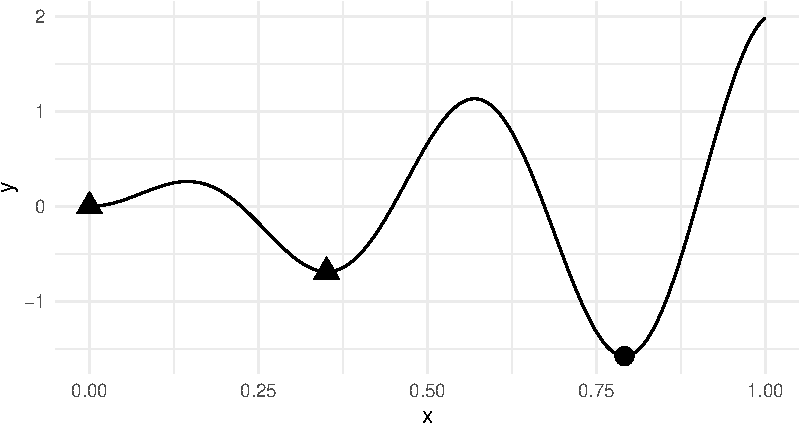
\includegraphics[width=1\textwidth,height=\textheight]{chapters/chapter5/advanced_tuning_methods_and_black_box_optimization_files/figure-pdf/fig-bayesian-optimization-sinusoidal-1.pdf}

}

\caption{\label{fig-bayesian-optimization-sinusoidal}Visualization of
the sinusoidal function. Local minima in triangles and global minimum in
the circle.}

\end{figure}

The global minimizer, 0.792, corresponds to the point of the domain with
the lowest function value:

\begin{Shaded}
\begin{Highlighting}[]
\NormalTok{xydt[y }\SpecialCharTok{==} \FunctionTok{min}\NormalTok{(y), ]}
\end{Highlighting}
\end{Shaded}

\begin{verbatim}
       x      y
1: 0.792 -1.577
\end{verbatim}

With the objective function defined, we can proceed to optimize it using
\texttt{OptimInstanceSingleCrit}. This class allows us to wrap the
objective function and explicitly specify a search space. The search
space defines the set of input values we want to optimize over, and it
is typically a subset or transformation of the domain, though by default
the entire domain is taken as the search space. In black box
optimization, it is common for the domain, and hence also the search
space, to have finite box constraints. Similarly to HPO, transformations
can sometimes be used to more efficiently search the space
(Section~\ref{sec-logarithmic-transformations}).

In the following, we use a simple random search to optimize the
sinusoidal function over the whole domain and inspect the result from
the \texttt{instance} in the usual way (Section~\ref{sec-tuner}).
Analogously to tuners, \texttt{Optimizer}s in \texttt{bbotk} are stored
in the
\href{https://bbotk.mlr-org.com/reference/mlr_optimizers.html}{\texttt{mlr\_optimizers}}
dictionary and can be constructed with
\href{https://bbotk.mlr-org.com/reference/opt.html}{\texttt{opt()}}\index{\texttt{opt()}}{\marginnote{\begin{footnotesize}\texttt{opt()}\end{footnotesize}}}.

\begin{Shaded}
\begin{Highlighting}[]
\NormalTok{instance }\OtherTok{=}\NormalTok{ OptimInstanceSingleCrit}\SpecialCharTok{$}\FunctionTok{new}\NormalTok{(objective,}
  \AttributeTok{search\_space =}\NormalTok{ domain,}
  \AttributeTok{terminator =} \FunctionTok{trm}\NormalTok{(}\StringTok{"evals"}\NormalTok{, }\AttributeTok{n\_evals =} \DecValTok{20}\NormalTok{))}
\NormalTok{optimizer }\OtherTok{=} \FunctionTok{opt}\NormalTok{(}\StringTok{"random\_search"}\NormalTok{, }\AttributeTok{batch\_size =} \DecValTok{20}\NormalTok{)}
\NormalTok{optimizer}\SpecialCharTok{$}\FunctionTok{optimize}\NormalTok{(instance)}
\end{Highlighting}
\end{Shaded}

Similarly to how we can use
\href{https://mlr3tuning.mlr-org.com/reference/tune.html}{\texttt{tune()}}
to construct a tuning instance, here we can use
\href{https://bbotk.mlr-org.com/reference/bb_optimize.html}{\texttt{bb\_optimize()}},
which returns a list with elements \texttt{"par"} (best found
parameters), \texttt{"val"} (optimal outcome), and \texttt{"instance"}
(the optimization instance); the values given as \texttt{"par"} and
\texttt{"val"} are the same as the values found in
\texttt{instance\$result}:

\begin{Shaded}
\begin{Highlighting}[]
\NormalTok{optimal }\OtherTok{=} \FunctionTok{bb\_optimize}\NormalTok{(objective, }\AttributeTok{method =} \StringTok{"random\_search"}\NormalTok{,}
  \AttributeTok{max\_evals =} \DecValTok{20}\NormalTok{)}
\NormalTok{optimal}\SpecialCharTok{$}\NormalTok{instance}\SpecialCharTok{$}\NormalTok{result}
\end{Highlighting}
\end{Shaded}

\begin{verbatim}
        x  x_domain      y
1: 0.7377 <list[1]> -1.158
\end{verbatim}

Now we have introduced the basic black box optimization setup, we can
introduce the building blocks of any Bayesian optimization algorithm.

\hypertarget{sec-bayesian-optimization-blocks}{%
\subsection{Building Blocks of Bayesian
Optimization}\label{sec-bayesian-optimization-blocks}}

Bayesian optimization (BO) is a global optimization algorithm that
usually follows the following process
(Figure~\ref{fig-optimization-loop}):

\begin{enumerate}
\def\labelenumi{\arabic{enumi}.}
\tightlist
\item
  Generate and evaluate an initial design\index{initial design}
\item
  Loop:

  \begin{enumerate}
  \def\labelenumii{\alph{enumii}.}
  \tightlist
  \item
    Fit a surrogate model\index{surrogate model} on the archive of all
    observations made so far to model the unknown black box function.
  \item
    Optimize an acquisition function\index{acquisition function} to
    determine which points of the search space are promising
    candidate(s) that should be evaluated next.
  \item
    Evaluate the next candidate(s) and update the archive of all
    observations made so far.
  \item
    Check if a given termination criterion is met, if not go back to
    (a).
  \end{enumerate}
\end{enumerate}

The acquisition function relies on the mean and standard deviation
prediction of the surrogate model and requires no evaluation of the true
black box function, making it comparably cheap to optimize. A good
acquisition function will balance \emph{exploiting} knowledge about
regions where we observed that performance is good and the surrogate
model has low uncertainty, with \emph{exploring} regions where it has
not yet evaluated points and as a result the uncertainty of the
surrogate model is high.

We refer to these elements as the `building blocks' of BO as it is a
highly modular algorithm; as long as the above structure is in place,
then the surrogate models, acquisition functions, and acquisition
function optimizers are all interchangeable to a certain extent. The
design of \texttt{mlr3mbo} reflects this modularity, with the base class
for
\href{https://mlr3mbo.mlr-org.com/reference/mlr_optimizers_mbo.html}{\texttt{OptimizerMbo}}
holding all the key elements: the BO algorithm loop structure
(\href{https://mlr3mbo.mlr-org.com/reference/loop_function.html}{\texttt{loop\_function}}),
\emph{surrogate} model
(\href{https://mlr3mbo.mlr-org.com/reference/Surrogate.html}{\texttt{Surrogate}}),
\emph{acquisition function}
(\href{https://mlr3mbo.mlr-org.com/reference/AcqFunction.html}{\texttt{AcqFunction}}),
and \emph{acquisition function optimizer}
(\href{https://mlr3mbo.mlr-org.com/reference/AcqOptimizer.html}{\texttt{AcqOptimizer}}).
In this section, we will provide a more detailed explanation of these
building blocks and explore their interplay and interaction during
optimization.

\begin{figure}

{\centering 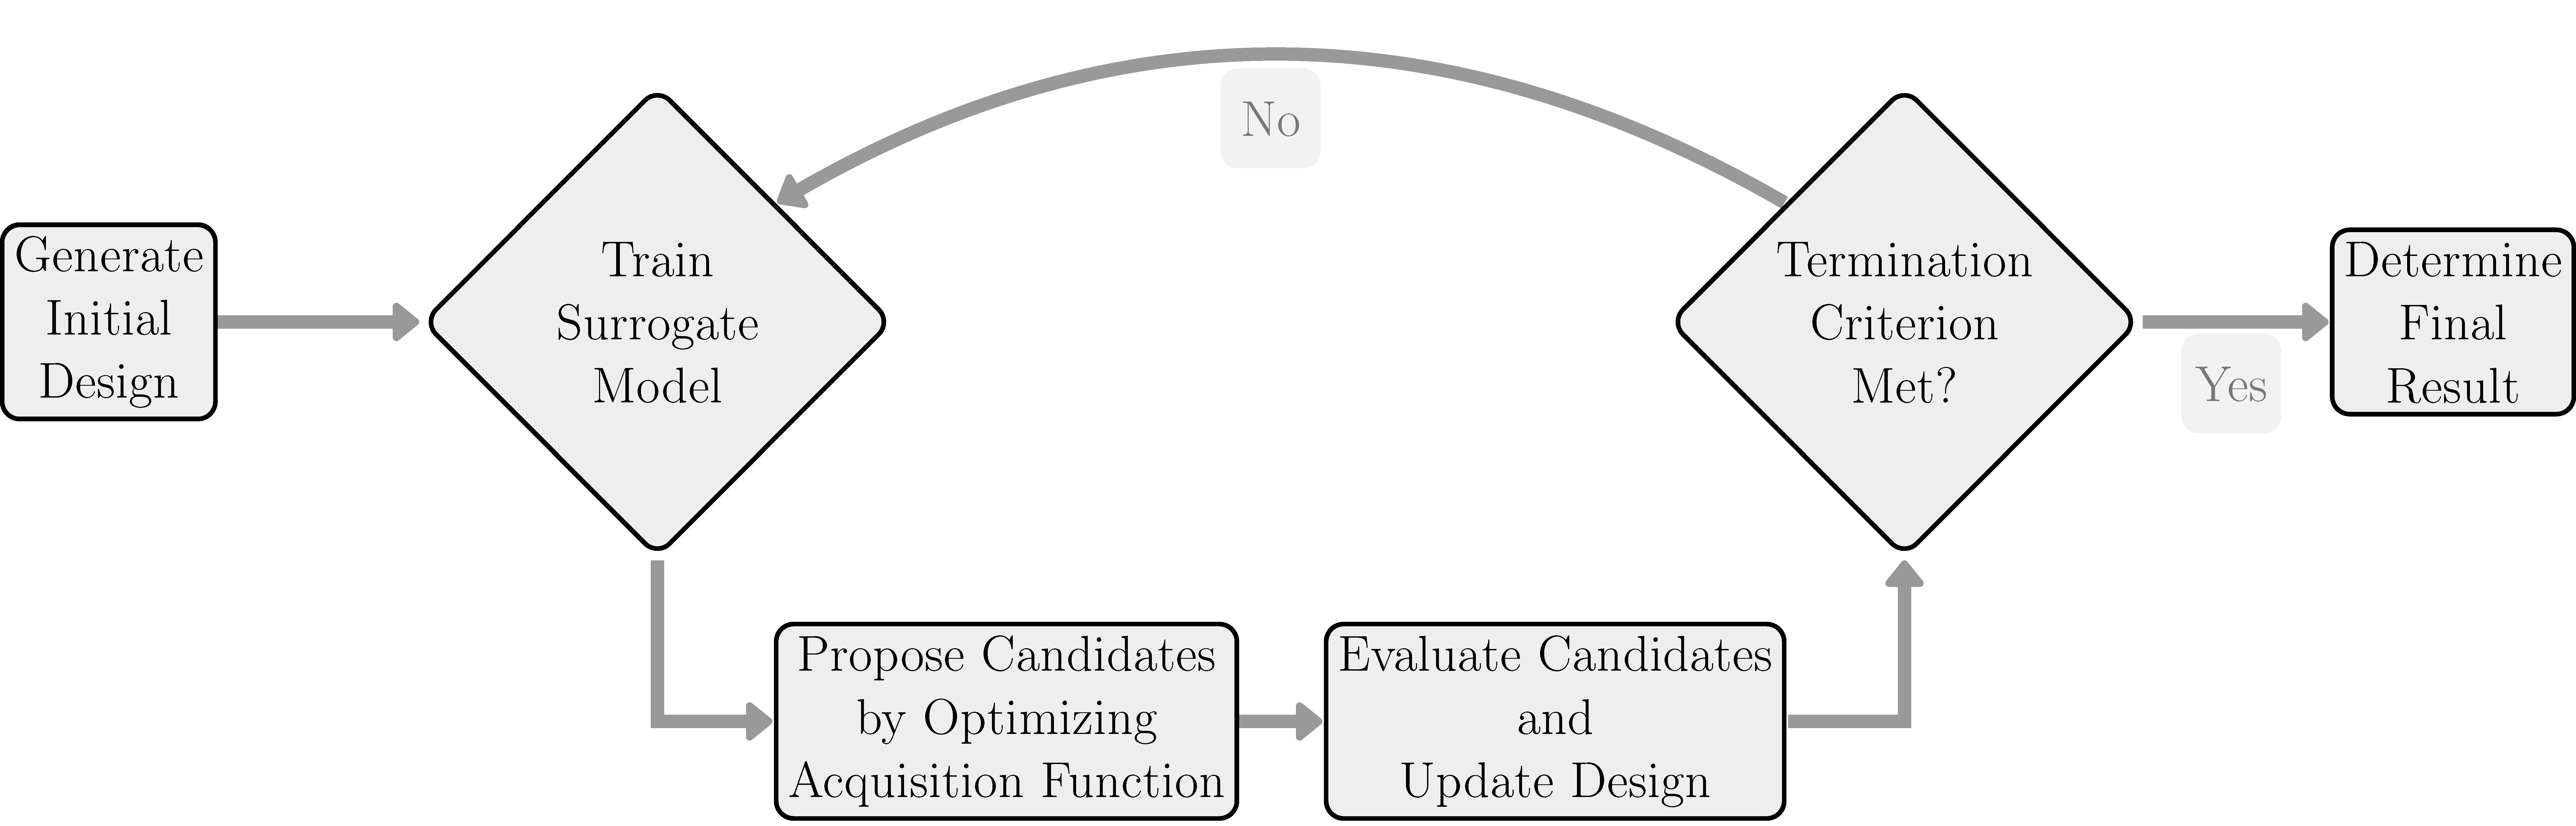
\includegraphics[width=0.8\textwidth,height=\textheight]{chapters/chapter5/Figures/mlr3book_figures-10.png}

}

\caption{\label{fig-optimization-loop}Bayesian optimization loop.}

\end{figure}

\hypertarget{sec-bayesian-optimization-initial}{%
\subsubsection{The Initial
Design}\label{sec-bayesian-optimization-initial}}

Before we can fit a surrogate model to model the unknown black box
function, we need data. The initial set of points that is evaluated
before a surrogate model can be fit is referred to as the initial
design\index{initial design}.

\texttt{mlr3mbo} allows you to either construct the initial design
manually or let a
\href{https://mlr3mbo.mlr-org.com/reference/loop_function.html}{\texttt{loop\_function}}
construct and evaluate this for you. In this section, we will
demonstrate the first method, which requires more user input but
therefore allows more control over the initial design.

A simple method to construct an initial design is to use one of the four
design generators in
\href{https://paradox.mlr-org.com}{\texttt{paradox}}\index{\texttt{paradox}}:

\begin{itemize}
\tightlist
\item
  \href{https://paradox.mlr-org.com/reference/generate_design_random.html}{\texttt{generate\_design\_random()}}:
  Generate points uniformly at random
\item
  \href{https://paradox.mlr-org.com/reference/generate_design_grid.html}{\texttt{generate\_design\_grid()}}:
  Generate points in a uniform-sized grid
\item
  \href{https://paradox.mlr-org.com/reference/generate_design_lhs.html}{\texttt{generate\_design\_lhs()}}:
  Latin hypercube sampling (Stein 1987)
\item
  \href{https://paradox.mlr-org.com/reference/generate_design_sobol.html}{\texttt{generate\_design\_sobol()}}:
  Sobol sequence (Niederreiter 1988)
\end{itemize}

Figure~\ref{fig-bayesian-optimization-designs} illustrates the
difference in generated designs from these four methods assuming an
initial design of size nine and a domain of two numeric variables from
\(0\) to \(1\). We already covered the difference between grid and
random designs in Section~\ref{sec-tuner}. An LHS design divides each
input variable into equally sized intervals (indicated by the horizontal
and vertical dotted lines in
Figure~\ref{fig-bayesian-optimization-designs}) and ensures that each
interval is represented by exactly one sample point, resulting in
uniform marginal distributions. Furthermore, in LHS designs the minimal
distance between two points is usually maximized, resulting in its
space-filling coverage of the space. The Sobol design works similarly to
LHS but can provide better coverage than LHS when the number of
dimensions is large. For this reason, LHS or Sobol designs are usually
recommended for BO, but usually the influence of the initial design will
be smaller compared to other design choices of BO. A random design might
work well-enough, but grid designs are usually discouraged.

\begin{figure}

{\centering 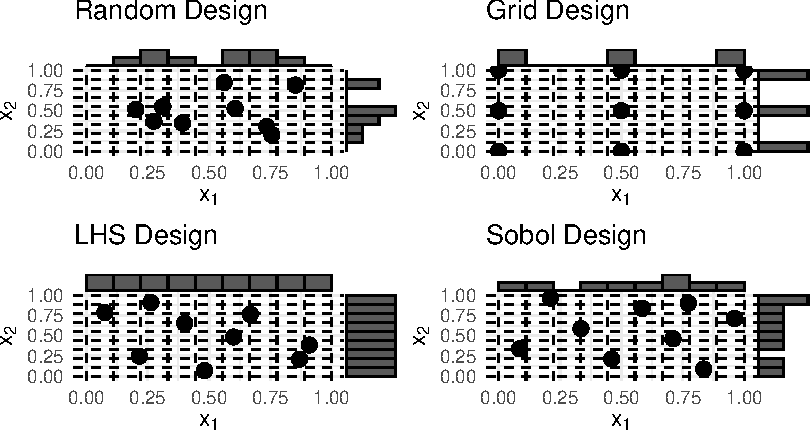
\includegraphics[width=1\textwidth,height=\textheight]{chapters/chapter5/advanced_tuning_methods_and_black_box_optimization_files/figure-pdf/fig-bayesian-optimization-designs-1.pdf}

}

\caption{\label{fig-bayesian-optimization-designs}Comparing different
samplers for constructing an initial design of nine points on a domain
of two numeric variables ranging from \(0\) to \(1\). Dotted horizontal
and vertical lines partition the domain into equally sized bins.
Histograms on the top and right visualize the marginal distributions of
the generated sample.}

\end{figure}

Whichever of these methods you choose, the result is a
\href{https://paradox.mlr-org.com/reference/Design.html}{\texttt{Design}}
object, which is mostly just a wrapper around a \texttt{data.table}:

\begin{Shaded}
\begin{Highlighting}[]
\NormalTok{sample\_domain }\OtherTok{=} \FunctionTok{ps}\NormalTok{(}\AttributeTok{x1 =} \FunctionTok{p\_dbl}\NormalTok{(}\DecValTok{0}\NormalTok{, }\DecValTok{1}\NormalTok{), }\AttributeTok{x2 =} \FunctionTok{p\_dbl}\NormalTok{(}\DecValTok{0}\NormalTok{, }\DecValTok{1}\NormalTok{))}
\FunctionTok{generate\_design\_random}\NormalTok{(sample\_domain, }\AttributeTok{n =} \DecValTok{3}\NormalTok{)}\SpecialCharTok{$}\NormalTok{data}
\end{Highlighting}
\end{Shaded}

\begin{verbatim}
       x1     x2
1: 0.9930 0.3773
2: 0.6782 0.4612
3: 0.4355 0.8019
\end{verbatim}

Therefore you could also specify a completely custom initial design by
defining your own \texttt{data.table}. Either way, when manually
constructing an initial design (as opposed to letting
\texttt{loop\_function} automate this), it needs to be evaluated on the
\href{https://bbotk.mlr-org.com/reference/OptimInstance.html}{\texttt{OptimInstance}}
before optimizing it. Returning to our running example of minimizing the
sinusoidal function, we will evaluate a custom initial design with
\texttt{\$eval\_batch()}:

\begin{Shaded}
\begin{Highlighting}[]
\NormalTok{instance }\OtherTok{=}\NormalTok{ OptimInstanceSingleCrit}\SpecialCharTok{$}\FunctionTok{new}\NormalTok{(objective,}
  \AttributeTok{terminator =} \FunctionTok{trm}\NormalTok{(}\StringTok{"evals"}\NormalTok{, }\AttributeTok{n\_evals =} \DecValTok{20}\NormalTok{))}
\NormalTok{design }\OtherTok{=} \FunctionTok{data.table}\NormalTok{(}\AttributeTok{x =} \FunctionTok{c}\NormalTok{(}\FloatTok{0.1}\NormalTok{, }\FloatTok{0.34}\NormalTok{, }\FloatTok{0.65}\NormalTok{, }\DecValTok{1}\NormalTok{))}
\NormalTok{instance}\SpecialCharTok{$}\FunctionTok{eval\_batch}\NormalTok{(design)}
\NormalTok{instance}\SpecialCharTok{$}\NormalTok{archive}\SpecialCharTok{$}\NormalTok{data}
\end{Highlighting}
\end{Shaded}

\begin{verbatim}
      x       y  x_domain           timestamp batch_nr
1: 0.10  0.1971 <list[1]> 2023-07-04 15:25:40        1
2: 0.34 -0.6792 <list[1]> 2023-07-04 15:25:40        1
3: 0.65  0.4148 <list[1]> 2023-07-04 15:25:40        1
4: 1.00  1.9812 <list[1]> 2023-07-04 15:25:40        1
\end{verbatim}

We can see how each point in our design was evaluated by the sinusoidal
function, giving us data we can now use to start the iterative BO
algorithm by fitting the surrogate model on that data.

\hypertarget{sec-bayesian-optimization-surrogate}{%
\subsubsection{Surrogate
Model}\label{sec-bayesian-optimization-surrogate}}

A surrogate model\index{surrogate model} wraps a regression learner that
models the unknown black box function based on observed data. In
\texttt{mlr3mbo}, the
\href{https://mlr3mbo.mlr-org.com/reference/SurrogateLearner.html}{\texttt{SurrogateLearner}}
is a higher-level R6 class inheriting from the base
\href{https://mlr3mbo.mlr-org.com/reference/Surrogate.html}{\texttt{Surrogate}}
class, designed to construct and manage the surrogate model, including
automatic construction of the \texttt{TaskRegr} that the learner should
be trained on at each iteration of the BO loop.

Any regression learner in \texttt{mlr3} can be used. However, most
acquisition functions depend on both mean and standard deviation
predictions from the surrogate model, the latter of which requires the
\texttt{"se"} \texttt{predict\_type} to be supported. Therefore not all
learners are suitable for all scenarios. Typical choices of regression
learners used as surrogate models include Gaussian
processes\index{Gaussian process} (\texttt{lrn("regr.km")}) for low to
medium dimensional numeric search spaces and random
forests\index{random forest} (e.g., \texttt{lrn("regr.ranger")}) for
higher dimensional mixed (and/or hierarchical) search spaces. A detailed
introduction to Gaussian processes can be found in Williams and
Rasmussen (2006) and an in-depth focus on Gaussian processes in the
context of surrogate models in BO is given in Garnett (2022). In this
example, we use a Gaussian process with Matérn 5/2 kernel, which uses
\texttt{BFGS} as an optimizer to find the optimal kernel parameters and
set \texttt{trace\ =\ FALSE} to prevent too much output during fitting.

\begin{Shaded}
\begin{Highlighting}[]
\NormalTok{lrn\_gp }\OtherTok{=} \FunctionTok{lrn}\NormalTok{(}\StringTok{"regr.km"}\NormalTok{, }\AttributeTok{covtype =} \StringTok{"matern5\_2"}\NormalTok{, }\AttributeTok{optim.method =} \StringTok{"BFGS"}\NormalTok{,}
  \AttributeTok{control =} \FunctionTok{list}\NormalTok{(}\AttributeTok{trace =} \ConstantTok{FALSE}\NormalTok{))}
\end{Highlighting}
\end{Shaded}

A \texttt{SurrogateLearner} can be constructed by passing a
\texttt{LearnerRegr} object to the sugar function
\texttt{srlrn()}\index{\texttt{srlrn()}}{\marginnote{\begin{footnotesize}srlrn()\end{footnotesize}}},
alongside the \texttt{archive} of the instance:

\begin{Shaded}
\begin{Highlighting}[]
\FunctionTok{library}\NormalTok{(mlr3mbo)}
\NormalTok{surrogate }\OtherTok{=} \FunctionTok{srlrn}\NormalTok{(lrn\_gp, }\AttributeTok{archive =}\NormalTok{ instance}\SpecialCharTok{$}\NormalTok{archive)}
\end{Highlighting}
\end{Shaded}

Internally, the regression learner is fit on a \texttt{TaskRegr} where
features are the variables of the domain and the target is the codomain,
the data is from the
\href{https://bbotk.mlr-org.com/reference/Archive.html}{\texttt{Archive}}
of the
\href{https://bbotk.mlr-org.com/reference/OptimInstance.html}{\texttt{OptimInstance}}
that is to be optimized.

In our running example we have already initialized our archive with the
initial design, so we can update our surrogate model, which essentially
fits the Gaussian process, note how we use \texttt{\$learner} to access
the wrapped model:

\begin{Shaded}
\begin{Highlighting}[]
\NormalTok{surrogate}\SpecialCharTok{$}\FunctionTok{update}\NormalTok{()}
\NormalTok{surrogate}\SpecialCharTok{$}\NormalTok{learner}\SpecialCharTok{$}\NormalTok{model}
\end{Highlighting}
\end{Shaded}

\begin{verbatim}

Call:
DiceKriging::km(design = data, response = task$truth(), covtype = "matern5_2", 
    optim.method = "BFGS", control = pv$control)

Trend  coeff.:
               Estimate
 (Intercept)     0.7899

Covar. type  : matern5_2 
Covar. coeff.:
               Estimate
    theta(x)     0.3014

Variance estimate: 1.07
\end{verbatim}

Having introduced the concept of a surrogate model, we can now move on
to the acquisition function, which makes use of the surrogate model
predictions to decide which candidate to evaluate next.

\hypertarget{sec-bayesian-optimization-acquisition}{%
\subsubsection{Acquisition
Function}\label{sec-bayesian-optimization-acquisition}}

Roughly speaking, an acquisition function\index{acquisition function}
relies on the prediction of a surrogate model and quantifies the
expected `utility' of each point of the search space if it were to be
evaluated in the next iteration.

A popular example is the expected improvement (Jones, Schonlau, and
Welch 1998), which tells us how much we can expect a candidate point to
improve over the best function value observed so far (the `incumbent'),
given the performance prediction of the surrogate model:

\[
\alpha_{\mathrm{EI}}(\mathbf{x}) = \mathbb{E} \left[ \max \left( f_{\mathrm{min}} - Y(\mathbf{x}), 0 \right) \right]
\]

Here, \(Y(\mathbf{x)}\) is the surrogate model prediction (a random
variable) for a given point \(\mathbf{x}\) (which when using a Gaussian
process follows a normal distribution) and \(f_{\mathrm{min}}\) is the
best function value observed so far (assuming minimization). Calculating
the expected improvement requires mean and standard deviation
predictions from the model.

In \texttt{mlr3mbo}, acquisition functions (of class
\href{https://mlr3mbo.mlr-org.com/reference/AcqFunction.html}{\texttt{AcqFunction}})
are stored in the
\href{https://mlr3mbo.mlr-org.com/reference/mlr_acqfunctions.html}{\texttt{mlr\_acqfunctions}}
dictionary and can be constructed with
\href{https://mlr3mbo.mlr-org.com/reference/acqf.html}{\texttt{acqf()}}\index{\texttt{acqf()}}{\marginnote{\begin{footnotesize}\texttt{acqf()}\end{footnotesize}}},
passing the key of the method you want to use and our surrogate learner.
In our running example, we will use the expected improvement
(\texttt{acqf("ei")}) to choose the next candidate for evaluation.
Before we can do that, we have to update (\texttt{\$update()}) the
\texttt{AcqFunction}'s view of the incumbent, to ensure it is still
using the best value observed so far.

\begin{Shaded}
\begin{Highlighting}[]
\NormalTok{acq\_function }\OtherTok{=} \FunctionTok{acqf}\NormalTok{(}\StringTok{"ei"}\NormalTok{, }\AttributeTok{surrogate =}\NormalTok{ surrogate)}
\NormalTok{acq\_function}\SpecialCharTok{$}\FunctionTok{update}\NormalTok{()}
\NormalTok{acq\_function}\SpecialCharTok{$}\NormalTok{y\_best}
\end{Highlighting}
\end{Shaded}

\begin{verbatim}
[1] -0.6792
\end{verbatim}

You can use \texttt{\$eval\_dt()} to evaluate the acquisition function
for the domain given as a \texttt{data.table}. In
Figure~\ref{fig-bayesian-optimization-ei} we evaluated the expected
improvement on a uniform grid of points between \(0\) and \(1\) using
the predicted mean and standard deviation from the Gaussian process. We
can see that the expected improvement is high in regions where the mean
prediction (gray dashed lines) of the Gaussian process is low, or where
the uncertainty is high.

\begin{Shaded}
\begin{Highlighting}[]
\NormalTok{xydt }\OtherTok{=} \FunctionTok{generate\_design\_grid}\NormalTok{(domain, }\AttributeTok{resolution =} \DecValTok{1001}\NormalTok{)}\SpecialCharTok{$}\NormalTok{data}
\CommentTok{\# evaluate our sinusoidal function}
\NormalTok{xydt[, y }\SpecialCharTok{:}\ErrorTok{=}\NormalTok{ objective}\SpecialCharTok{$}\FunctionTok{eval\_dt}\NormalTok{(xydt)}\SpecialCharTok{$}\NormalTok{y]}
\CommentTok{\# evaluate expected improvement}
\NormalTok{xydt[, ei }\SpecialCharTok{:}\ErrorTok{=}\NormalTok{  acq\_function}\SpecialCharTok{$}\FunctionTok{eval\_dt}\NormalTok{(xydt[, }\StringTok{"x"}\NormalTok{])]}
\CommentTok{\# make predictions from our data}
\NormalTok{xydt[, }\FunctionTok{c}\NormalTok{(}\StringTok{"mean"}\NormalTok{, }\StringTok{"se"}\NormalTok{) }\SpecialCharTok{:}\ErrorTok{=}\NormalTok{  surrogate}\SpecialCharTok{$}\FunctionTok{predict}\NormalTok{(xydt[, }\StringTok{"x"}\NormalTok{])]}
\NormalTok{xydt[}\DecValTok{1}\SpecialCharTok{:}\DecValTok{3}\NormalTok{]}
\end{Highlighting}
\end{Shaded}

\begin{verbatim}
       x        y        ei   mean     se
1: 0.000 0.000000 4.642e-05 0.5191 0.3632
2: 0.001 0.000028 4.171e-05 0.5166 0.3597
3: 0.002 0.000112 3.738e-05 0.5142 0.3562
\end{verbatim}

\begin{Shaded}
\begin{Highlighting}[]
\FunctionTok{ggplot}\NormalTok{(xydt, }\AttributeTok{mapping =} \FunctionTok{aes}\NormalTok{(}\AttributeTok{x =}\NormalTok{ x, }\AttributeTok{y =}\NormalTok{ y)) }\SpecialCharTok{+}
  \FunctionTok{geom\_point}\NormalTok{(}\AttributeTok{size =} \DecValTok{2}\NormalTok{, }\AttributeTok{data =}\NormalTok{ instance}\SpecialCharTok{$}\NormalTok{archive}\SpecialCharTok{$}\NormalTok{data) }\SpecialCharTok{+}
  \FunctionTok{geom\_line}\NormalTok{() }\SpecialCharTok{+}
  \FunctionTok{geom\_line}\NormalTok{(}\FunctionTok{aes}\NormalTok{(}\AttributeTok{y =}\NormalTok{ mean), }\AttributeTok{colour =} \StringTok{"gray"}\NormalTok{, }\AttributeTok{linetype =} \DecValTok{2}\NormalTok{) }\SpecialCharTok{+}
  \FunctionTok{geom\_ribbon}\NormalTok{(}\FunctionTok{aes}\NormalTok{(}\AttributeTok{min =}\NormalTok{ mean }\SpecialCharTok{{-}}\NormalTok{ se, }\AttributeTok{max =}\NormalTok{ mean }\SpecialCharTok{+}\NormalTok{ se),}
    \AttributeTok{fill =} \StringTok{"gray"}\NormalTok{, }\AttributeTok{alpha =} \FloatTok{0.3}\NormalTok{) }\SpecialCharTok{+}
  \FunctionTok{geom\_line}\NormalTok{(}\FunctionTok{aes}\NormalTok{(}\AttributeTok{y =}\NormalTok{ ei }\SpecialCharTok{*} \DecValTok{40}\NormalTok{), }\AttributeTok{linewidth =} \DecValTok{1}\NormalTok{, }\AttributeTok{colour =} \StringTok{"darkgray"}\NormalTok{) }\SpecialCharTok{+}
  \FunctionTok{scale\_y\_continuous}\NormalTok{(}\StringTok{"y"}\NormalTok{,}
    \AttributeTok{sec.axis =} \FunctionTok{sec\_axis}\NormalTok{(}\SpecialCharTok{\textasciitilde{}}\NormalTok{ . }\SpecialCharTok{*} \FloatTok{0.025}\NormalTok{, }\AttributeTok{name =} \StringTok{"EI"}\NormalTok{,}
      \AttributeTok{breaks =} \FunctionTok{c}\NormalTok{(}\DecValTok{0}\NormalTok{, }\FloatTok{0.025}\NormalTok{, }\FloatTok{0.05}\NormalTok{))) }\SpecialCharTok{+}
  \FunctionTok{theme\_minimal}\NormalTok{()}
\end{Highlighting}
\end{Shaded}

\begin{figure}[H]

{\centering 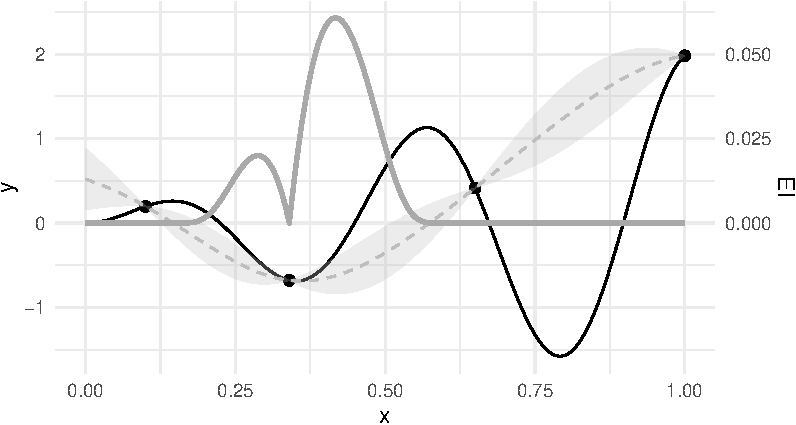
\includegraphics[width=1\textwidth,height=\textheight]{chapters/chapter5/advanced_tuning_methods_and_black_box_optimization_files/figure-pdf/fig-bayesian-optimization-ei-1.pdf}

}

\caption{\label{fig-bayesian-optimization-ei}Expected improvement (solid
dark gray line) based on the mean and uncertainty prediction (dashed
gray line) of the Gaussian process surrogate model trained on an initial
design of four points (black). Ribbons represent the mean plus minus the
standard deviation prediction.}

\end{figure}

We will now proceed to optimize the acquisition function itself to find
the candidate with the largest expected improvement.

\hypertarget{sec-bayesian-optimization-acquisitionopt}{%
\subsubsection{Acquisition Function
Optimizer}\label{sec-bayesian-optimization-acquisitionopt}}

An acquisition function optimizer\index{acquisition function optimizer}
of class
\href{https://mlr3mbo.mlr-org.com/reference/AcqOptimizer.html}{\texttt{AcqOptimizer}}\index{\texttt{AcqOptimizer}}{\marginnote{\begin{footnotesize}\texttt{AcqOptimizer}\end{footnotesize}}}
is used to optimize the acquisition function by efficiently searching
the space of potential candidates within a limited computational budget.

Due to the non-convex nature of most commonly used acquisition functions
(Garnett 2022) it is typical to employ global optimization techniques
for acquisition function optimization. Widely used approaches for
optimizing acquisition functions include derivative-free global
optimization methods like branch and bound algorithms, such as the
DIRECT\index{DIRECT} algorithm (Jones, Perttunen, and Stuckman 1993), as
well as multi-start local optimization methods, such as running the
L-BFGS-B\index{L-BFGS-B} algorithm (Byrd et al. 1995) or a local search
multiple times from various starting points (J. Kim and Choi 2021).
Consequently the optimization problem of the acquisition function can be
handled as a black box optimization problem itself, but a much cheaper
one than the original.

\texttt{AcqOptimizer} objects are constructed with
\href{https://mlr3mbo.mlr-org.com/reference/acqo.html}{\texttt{acqo()}}\index{\texttt{acqo()}}{\marginnote{\begin{footnotesize}\texttt{acqo()}\end{footnotesize}}},
which takes as input a
\href{https://bbotk.mlr-org.com/reference/Optimizer.html}{\texttt{Optimizer}},
a
\href{https://bbotk.mlr-org.com/reference/Terminator.html}{\texttt{Terminator}},
and the acquisition function. Optimizers are stored in the
\href{https://bbotk.mlr-org.com/reference/mlr_optimizers.html}{\texttt{mlr\_optimizers}}
dictionary and can be constructed with the sugar function
\href{https://bbotk.mlr-org.com/reference/opt.html}{\texttt{opt()}}\index{\texttt{opt()}}{\marginnote{\begin{footnotesize}\texttt{opt()}\end{footnotesize}}}.
The terminators are the same as those introduced in
Section~\ref{sec-terminator}.

Below we use the DIRECT algorithm and we terminate the acquisition
function optimization if there is no improvement of at least
\texttt{1e-5} for \texttt{100} iterations. The \texttt{\$optimize()}
method optimizes the acquisition function and returns the next
candidate.

\begin{Shaded}
\begin{Highlighting}[]
\NormalTok{acq\_optimizer }\OtherTok{=} \FunctionTok{acqo}\NormalTok{(}
  \AttributeTok{optimizer =} \FunctionTok{opt}\NormalTok{(}\StringTok{"nloptr"}\NormalTok{, }\AttributeTok{algorithm =} \StringTok{"NLOPT\_GN\_ORIG\_DIRECT"}\NormalTok{),}
  \AttributeTok{terminator =} \FunctionTok{trm}\NormalTok{(}\StringTok{"stagnation"}\NormalTok{, }\AttributeTok{iters =} \DecValTok{100}\NormalTok{, }\AttributeTok{threshold =} \FloatTok{1e{-}5}\NormalTok{),}
  \AttributeTok{acq\_function =}\NormalTok{ acq\_function}
\NormalTok{)}

\NormalTok{candidate }\OtherTok{=}\NormalTok{ acq\_optimizer}\SpecialCharTok{$}\FunctionTok{optimize}\NormalTok{()}
\NormalTok{candidate}
\end{Highlighting}
\end{Shaded}

\begin{verbatim}
        x  x_domain  acq_ei .already_evaluated
1: 0.4173 <list[1]> 0.06074              FALSE
\end{verbatim}

We have now shown how to run a single iteration of the BO algorithm loop
manually. In practice, one would use
\href{https://mlr3mbo.mlr-org.com/reference/mlr_optimizers_mbo.html}{\texttt{OptimizerMbo}}
to put all these pieces together to automate the process. Before
demonstrating this class we will first take a step back and introduce
the \texttt{loop\_function} which tells the algorithm how it should be
run.

\hypertarget{sec-bayesian-optimization-loop}{%
\subsubsection{Using and Building Loop
Functions}\label{sec-bayesian-optimization-loop}}

The
\href{https://mlr3mbo.mlr-org.com/reference/loop_function.html}{\texttt{loop\_function}}\index{\texttt{loop\_function}}
determines the behavior of the BO algorithm on a global level, i.e., how
to define the subroutine that is performed at each iteration to generate
new candidates for evaluation. Loop functions\index{loop functions} are
relatively simple functions that take as input the classes that we have
just discussed and define the BO loop. Loop functions are stored in the
\href{https://mlr3mbo.mlr-org.com/reference/mlr_loop_functions.html}{\texttt{mlr\_loop\_functions}}
dictionary. As these are \texttt{S3} (not \texttt{R6}) classes, they can
be simply loaded by just referencing the \texttt{key} (i.e., there is no
constructor required).

\begin{Shaded}
\begin{Highlighting}[]
\FunctionTok{as.data.table}\NormalTok{(mlr\_loop\_functions)[, .(key, label, instance)]}
\end{Highlighting}
\end{Shaded}

\begin{verbatim}
               key                         label    instance
1:    bayesopt_ego Efficient Global Optimization single-crit
2:    bayesopt_emo           Multi-Objective EGO  multi-crit
3:   bayesopt_mpcl      Multipoint Constant Liar single-crit
4: bayesopt_parego                        ParEGO  multi-crit
5: bayesopt_smsego                       SMS-EGO  multi-crit
\end{verbatim}

You could pick and use one of the loop functions included in the
dictionary above, or you can write your own for finer control over the
BO process. A common choice of loop function is the Efficient Global
Optimization\index{efficient global optimization} (EGO) algorithm
(Jones, Schonlau, and Welch 1998)
(\href{https://mlr3mbo.mlr-org.com/reference/mlr_loop_functions_ego.html}{\texttt{bayesopt\_ego()}}).
A simplified version of this code is shown at the end of this section,
both to help demonstrate the EGO algorithm, and to give an example of
how to write a custom BO variant yourself. In short, the code sets up
the relevant components discussed above and then loops the steps above:
1) update the surrogate model 2) update the acquisition function 3)
optimize the acquisition function to yield a new candidate 4) evaluate
the candidate and add it to the archive. If there is an error during the
loop then a fallback is used where the next candidate is proposed
uniformly at random, ensuring that the process continues even in the
presence of potential issues, we will return to this in
Section~\ref{sec-practical-bayesian-optimization}.

\begin{Shaded}
\begin{Highlighting}[]
\NormalTok{my\_simple\_ego }\OtherTok{=} \ControlFlowTok{function}\NormalTok{(}
\NormalTok{    instance,}
\NormalTok{    surrogate,}
\NormalTok{    acq\_function,}
\NormalTok{    acq\_optimizer,}
\NormalTok{    init\_design\_size}
\NormalTok{  ) \{}

  \CommentTok{\# setting up the building blocks}
\NormalTok{  surrogate}\SpecialCharTok{$}\NormalTok{archive }\OtherTok{=}\NormalTok{ instance}\SpecialCharTok{$}\NormalTok{archive }\CommentTok{\# archive}
\NormalTok{  acq\_function}\SpecialCharTok{$}\NormalTok{surrogate }\OtherTok{=}\NormalTok{ surrogate }\CommentTok{\# surrogate model}
\NormalTok{  acq\_optimizer}\SpecialCharTok{$}\NormalTok{acq\_function }\OtherTok{=}\NormalTok{ acq\_function }\CommentTok{\# acquisition function}

\NormalTok{  search\_space }\OtherTok{=}\NormalTok{ instance}\SpecialCharTok{$}\NormalTok{search\_space}

  \CommentTok{\# initial design}
\NormalTok{  design }\OtherTok{=} \FunctionTok{generate\_design\_sobol}\NormalTok{(}
\NormalTok{    search\_space, }\AttributeTok{n =}\NormalTok{ init\_design\_size)}\SpecialCharTok{$}\NormalTok{data}
\NormalTok{  instance}\SpecialCharTok{$}\FunctionTok{eval\_batch}\NormalTok{(design)}

  \CommentTok{\# MBO loop}
  \ControlFlowTok{repeat}\NormalTok{ \{}
\NormalTok{    candidate }\OtherTok{=} \FunctionTok{tryCatch}\NormalTok{(\{}
      \CommentTok{\# update the surrogate model}
\NormalTok{      acq\_function}\SpecialCharTok{$}\NormalTok{surrogate}\SpecialCharTok{$}\FunctionTok{update}\NormalTok{()}
      \CommentTok{\# update the acquisition function}
\NormalTok{      acq\_function}\SpecialCharTok{$}\FunctionTok{update}\NormalTok{()}
      \CommentTok{\# optimize the acquisition function to yield a new candidate}
\NormalTok{      acq\_optimizer}\SpecialCharTok{$}\FunctionTok{optimize}\NormalTok{()}
\NormalTok{    \}, }\AttributeTok{mbo\_error =} \ControlFlowTok{function}\NormalTok{(mbo\_error\_condition) \{}
      \FunctionTok{generate\_design\_random}\NormalTok{(search\_space, }\AttributeTok{n =}\NormalTok{ 1L)}\SpecialCharTok{$}\NormalTok{data}
\NormalTok{    \})}

    \CommentTok{\# evaluate the candidate and add it to the archive}
    \FunctionTok{tryCatch}\NormalTok{(\{}
\NormalTok{      instance}\SpecialCharTok{$}\FunctionTok{eval\_batch}\NormalTok{(candidate)}
\NormalTok{    \}, }\AttributeTok{terminated\_error =} \ControlFlowTok{function}\NormalTok{(cond) \{}
      \CommentTok{\# $eval\_batch() throws a terminated\_error if the instance is}
      \CommentTok{\# already terminated, e.g. because of timeout.}
\NormalTok{    \})}
    \ControlFlowTok{if}\NormalTok{ (instance}\SpecialCharTok{$}\NormalTok{is\_terminated) }\ControlFlowTok{break}
\NormalTok{  \}}

  \FunctionTok{return}\NormalTok{(instance)}
\NormalTok{\}}
\end{Highlighting}
\end{Shaded}

We are now ready to put everything together to automate the BO process.

\hypertarget{sec-bayesian-black-box-optimization}{%
\subsection{Automating BO with
OptimizerMbo}\label{sec-bayesian-black-box-optimization}}

\href{https://mlr3mbo.mlr-org.com/reference/mlr_optimizers_mbo.html}{\texttt{OptimizerMbo}}
can be used to assemble the building blocks described above into a
single object that can then be used for optimization. We use the
\texttt{bayesopt\_ego} loop function provided by
\texttt{mlr\_loop\_functions}, which works similarly to the code shown
above but takes more care to offer sensible default values for its
arguments and handle edge cases correctly. You do not need to pass any
of these building blocks to each other manually as the
\href{https://bbotk.mlr-org.com/reference/opt.html}{\texttt{opt()}}\index{\texttt{opt()}}{\marginnote{\begin{footnotesize}\texttt{opt()}\end{footnotesize}}}
constructor will do this for you:

\begin{Shaded}
\begin{Highlighting}[]
\NormalTok{bayesopt\_ego }\OtherTok{=}\NormalTok{ mlr\_loop\_functions}\SpecialCharTok{$}\FunctionTok{get}\NormalTok{(}\StringTok{"bayesopt\_ego"}\NormalTok{)}
\NormalTok{surrogate }\OtherTok{=} \FunctionTok{srlrn}\NormalTok{(}\FunctionTok{lrn}\NormalTok{(}\StringTok{"regr.km"}\NormalTok{, }\AttributeTok{covtype =} \StringTok{"matern5\_2"}\NormalTok{,}
  \AttributeTok{optim.method =} \StringTok{"BFGS"}\NormalTok{, }\AttributeTok{control =} \FunctionTok{list}\NormalTok{(}\AttributeTok{trace =} \ConstantTok{FALSE}\NormalTok{)))}
\NormalTok{acq\_function }\OtherTok{=} \FunctionTok{acqf}\NormalTok{(}\StringTok{"ei"}\NormalTok{)}
\NormalTok{acq\_optimizer }\OtherTok{=} \FunctionTok{acqo}\NormalTok{(}\FunctionTok{opt}\NormalTok{(}\StringTok{"nloptr"}\NormalTok{, }\AttributeTok{algorithm =} \StringTok{"NLOPT\_GN\_ORIG\_DIRECT"}\NormalTok{),}
  \AttributeTok{terminator =} \FunctionTok{trm}\NormalTok{(}\StringTok{"stagnation"}\NormalTok{, }\AttributeTok{iters =} \DecValTok{100}\NormalTok{, }\AttributeTok{threshold =} \FloatTok{1e{-}5}\NormalTok{))}

\NormalTok{optimizer }\OtherTok{=} \FunctionTok{opt}\NormalTok{(}\StringTok{"mbo"}\NormalTok{,}
  \AttributeTok{loop\_function =}\NormalTok{ bayesopt\_ego,}
  \AttributeTok{surrogate =}\NormalTok{ surrogate,}
  \AttributeTok{acq\_function =}\NormalTok{ acq\_function,}
  \AttributeTok{acq\_optimizer =}\NormalTok{ acq\_optimizer)}
\end{Highlighting}
\end{Shaded}

\begin{tcolorbox}[enhanced jigsaw, opacitybacktitle=0.6, rightrule=.15mm, opacityback=0, arc=.35mm, breakable, titlerule=0mm, colframe=quarto-callout-tip-color-frame, coltitle=black, bottomrule=.15mm, toprule=.15mm, colback=white, colbacktitle=quarto-callout-tip-color!10!white, bottomtitle=1mm, toptitle=1mm, title=\textcolor{quarto-callout-tip-color}{\faLightbulb}\hspace{0.5em}{Loop Function Arguments}, leftrule=.75mm, left=2mm]

Additional arguments for customizing certain loop functions can be
passed through with the \texttt{args} parameter of \texttt{opt()}.

\end{tcolorbox}

In this example, we will use the same initial design that we created
before and will optimize our sinusoidal function using
\texttt{\$optimize()}:

\begin{Shaded}
\begin{Highlighting}[]
\NormalTok{instance }\OtherTok{=}\NormalTok{ OptimInstanceSingleCrit}\SpecialCharTok{$}\FunctionTok{new}\NormalTok{(objective,}
  \AttributeTok{terminator =} \FunctionTok{trm}\NormalTok{(}\StringTok{"evals"}\NormalTok{, }\AttributeTok{n\_evals =} \DecValTok{20}\NormalTok{))}
\NormalTok{design }\OtherTok{=} \FunctionTok{data.table}\NormalTok{(}\AttributeTok{x =} \FunctionTok{c}\NormalTok{(}\FloatTok{0.1}\NormalTok{, }\FloatTok{0.34}\NormalTok{, }\FloatTok{0.65}\NormalTok{, }\DecValTok{1}\NormalTok{))}
\NormalTok{instance}\SpecialCharTok{$}\FunctionTok{eval\_batch}\NormalTok{(design)}
\NormalTok{optimizer}\SpecialCharTok{$}\FunctionTok{optimize}\NormalTok{(instance)}
\end{Highlighting}
\end{Shaded}

\begin{verbatim}
        x  x_domain      y
1: 0.7922 <list[1]> -1.577
\end{verbatim}

Using only a few evaluations, BO comes close to the true global optimum
(0.792). Figure~\ref{fig-bayesian-optimization-sampling} shows the
sampling trajectory of candidates as the algorithm progressed, we can
see that focus is increasingly given to more regions around the global
optimum. However, even in later optimization stages, the algorithm still
explores new areas, illustrating that the expected improvement
acquisition function indeed balances exploration and exploitation as we
required.

\begin{figure}

{\centering 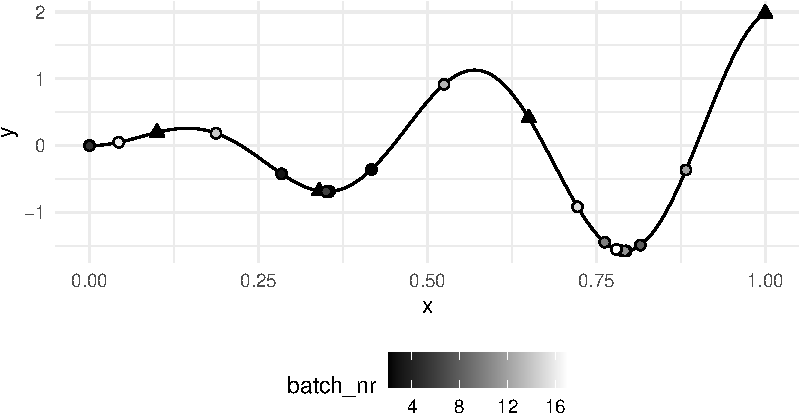
\includegraphics[width=1\textwidth,height=\textheight]{chapters/chapter5/advanced_tuning_methods_and_black_box_optimization_files/figure-pdf/fig-bayesian-optimization-sampling-1.pdf}

}

\caption{\label{fig-bayesian-optimization-sampling}Sampling trajectory
of the BO algorithm. Points of the initial design in black triangles.
Sampled points are in dots with color progressing from black to white as
the algorithm progresses.}

\end{figure}

If we replicate running our BO algorithm ten times (with random initial
designs and varying random seeds) and compare this to a random search,
we can see that BO indeed performs much better and on average reaches
the global optimum after around 15 function evaluations
(Figure~\ref{fig-bayesian-sinusoidal_bo_rs}). As expected, the
performance for the initial design size is close to the performance of
the random search.

\begin{figure}

{\centering 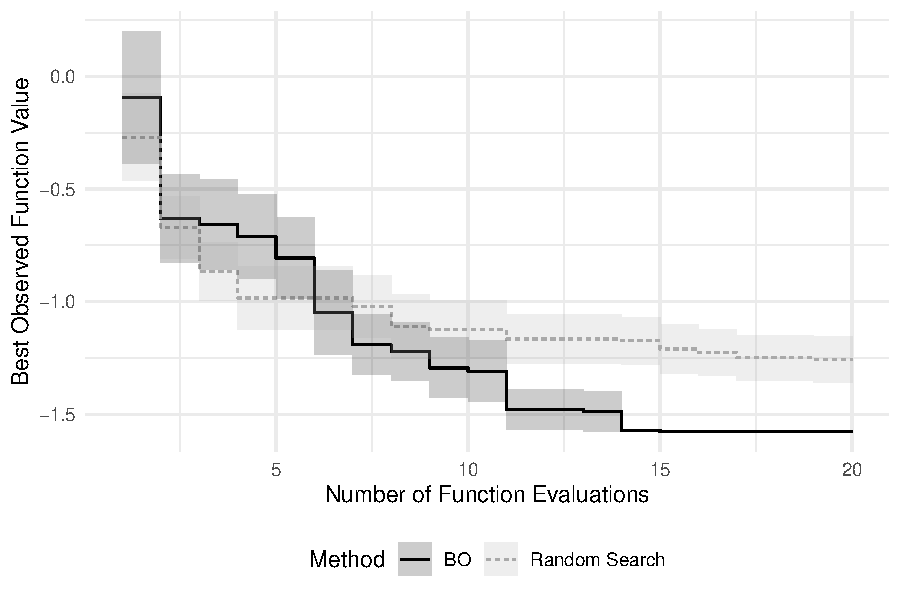
\includegraphics[width=1\textwidth,height=\textheight]{chapters/chapter5/Figures/bo_1d_sinusoidal_bo_rs.pdf}

}

\caption{\label{fig-bayesian-sinusoidal_bo_rs}Anytime performance of BO
and random search on the 1D sinusoidal function given a budget of 20
function evaluations. Solid line depicts the best observed target value
averaged over 10 replications. Ribbons represent standard errors.}

\end{figure}

\hypertarget{sec-bayesian-tuning}{%
\subsection{Bayesian Optimization for HPO}\label{sec-bayesian-tuning}}

\texttt{mlr3mbo} can be used for HPO by making use of
\href{https://mlr3mbo.mlr-org.com/reference/mlr_tuners_mbo.html}{\texttt{TunerMbo}}\index{\texttt{TunerMbo}}{\marginnote{\begin{footnotesize}\texttt{TunerMbo}\end{footnotesize}}},
which is a wrapper around
\href{https://mlr3mbo.mlr-org.com/reference/mlr_optimizers_mbo.html}{\texttt{OptimizerMbo}}
and works in the exact same way. As an example, below we will tune the
\texttt{cost} and \texttt{gamma} parameters of
\texttt{lrn("classif.svm")} with a radial kernel on
\texttt{tsk("sonar")} with three-fold CV. We set up \texttt{tnr("mbo")}
using the same objects constructed above and then run our tuning
experiment as usual:

\begin{Shaded}
\begin{Highlighting}[]
\NormalTok{tuner }\OtherTok{=} \FunctionTok{tnr}\NormalTok{(}\StringTok{"mbo"}\NormalTok{,}
  \AttributeTok{loop\_function =}\NormalTok{ bayesopt\_ego,}
  \AttributeTok{surrogate =}\NormalTok{ surrogate,}
  \AttributeTok{acq\_function =}\NormalTok{ acq\_function,}
  \AttributeTok{acq\_optimizer =}\NormalTok{ acq\_optimizer)}

\NormalTok{lrn\_svm }\OtherTok{=} \FunctionTok{lrn}\NormalTok{(}\StringTok{"classif.svm"}\NormalTok{, }\AttributeTok{kernel =} \StringTok{"radial"}\NormalTok{,}
  \AttributeTok{type =} \StringTok{"C{-}classification"}\NormalTok{,}
  \AttributeTok{cost  =} \FunctionTok{to\_tune}\NormalTok{(}\FloatTok{1e{-}5}\NormalTok{, }\FloatTok{1e5}\NormalTok{, }\AttributeTok{logscale =} \ConstantTok{TRUE}\NormalTok{),}
  \AttributeTok{gamma =} \FunctionTok{to\_tune}\NormalTok{(}\FloatTok{1e{-}5}\NormalTok{, }\FloatTok{1e5}\NormalTok{, }\AttributeTok{logscale =} \ConstantTok{TRUE}\NormalTok{)}
\NormalTok{)}

\NormalTok{instance }\OtherTok{=} \FunctionTok{tune}\NormalTok{(tuner, }\FunctionTok{tsk}\NormalTok{(}\StringTok{"sonar"}\NormalTok{), lrn\_svm, }\FunctionTok{rsmp}\NormalTok{(}\StringTok{"cv"}\NormalTok{, }\AttributeTok{folds =} \DecValTok{3}\NormalTok{),}
  \FunctionTok{msr}\NormalTok{(}\StringTok{"classif.ce"}\NormalTok{), }\DecValTok{25}\NormalTok{)}

\NormalTok{instance}\SpecialCharTok{$}\NormalTok{result}
\end{Highlighting}
\end{Shaded}

\begin{verbatim}
    cost  gamma learner_param_vals  x_domain classif.ce
1: 11.51 -4.075          <list[4]> <list[2]>     0.1489
\end{verbatim}

Multi-objective tuning is also possible with BO with algorithms using
many different design choices, for example, whether they use a
scalarization approach of objectives and only rely on a single surrogate
model, or fit a surrogate model for each objective. More details on
multi-objective BO can for example be found in Horn et al. (2015) or
Morales-Hernández, Van Nieuwenhuyse, and Rojas Gonzalez (2022).

Below we will illustrate multi-objective tuning using the ParEGO
(Knowles 2006) loop function. ParEGO
(\href{https://mlr3mbo.mlr-org.com/reference/mlr_loop_functions_parego.html}{\texttt{bayesopt\_parego()}})
tackles multi-objective BO via a randomized scalarization approach and
models a single scalarized objective function via a single surrogate
model and then proceeds to find the next candidate for evaluation making
use of a standard single-objective acquisition function such as the
expected improvement. Other compatible loop functions can be found by
looking at the \texttt{"instance"} column of
\href{https://mlr3mbo.mlr-org.com/reference/mlr_loop_functions.html}{\texttt{mlr\_loop\_functions}}.
We will tune three parameters of a decision tree with respect to the
true positive (maximize) and false positive (minimize) rates, the Pareto
front\index{Pareto front} is visualized in
Figure~\ref{fig-pareto-bayesopt}.

\begin{Shaded}
\begin{Highlighting}[]
\NormalTok{tuner }\OtherTok{=} \FunctionTok{tnr}\NormalTok{(}\StringTok{"mbo"}\NormalTok{,}
  \AttributeTok{loop\_function =}\NormalTok{ bayesopt\_parego,}
  \AttributeTok{surrogate =}\NormalTok{ surrogate,}
  \AttributeTok{acq\_function =}\NormalTok{ acq\_function,}
  \AttributeTok{acq\_optimizer =}\NormalTok{ acq\_optimizer)}

\NormalTok{lrn\_rpart }\OtherTok{=} \FunctionTok{lrn}\NormalTok{(}\StringTok{"classif.rpart"}\NormalTok{,}
  \AttributeTok{cp =} \FunctionTok{to\_tune}\NormalTok{(}\FloatTok{1e{-}04}\NormalTok{, }\FloatTok{1e{-}1}\NormalTok{),}
  \AttributeTok{minsplit =} \FunctionTok{to\_tune}\NormalTok{(}\DecValTok{2}\NormalTok{, }\DecValTok{64}\NormalTok{),}
  \AttributeTok{maxdepth =} \FunctionTok{to\_tune}\NormalTok{(}\DecValTok{1}\NormalTok{, }\DecValTok{30}\NormalTok{)}
\NormalTok{)}

\NormalTok{instance }\OtherTok{=} \FunctionTok{tune}\NormalTok{(tuner, }\FunctionTok{tsk}\NormalTok{(}\StringTok{"sonar"}\NormalTok{), lrn\_svm, }\FunctionTok{rsmp}\NormalTok{(}\StringTok{"cv"}\NormalTok{, }\AttributeTok{folds =} \DecValTok{3}\NormalTok{),}
  \FunctionTok{msrs}\NormalTok{(}\FunctionTok{c}\NormalTok{(}\StringTok{"classif.tpr"}\NormalTok{, }\StringTok{"classif.fpr"}\NormalTok{)), }\DecValTok{25}\NormalTok{)}
\end{Highlighting}
\end{Shaded}

\begin{figure}

{\centering 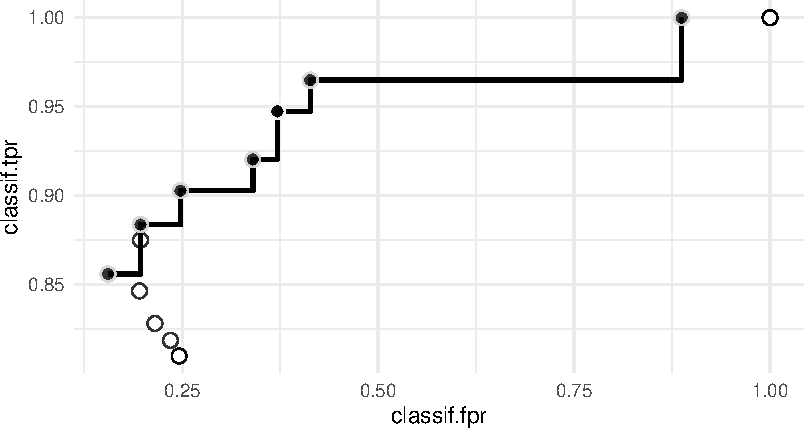
\includegraphics[width=1\textwidth,height=\textheight]{chapters/chapter5/advanced_tuning_methods_and_black_box_optimization_files/figure-pdf/fig-pareto-bayesopt-1.pdf}

}

\caption{\label{fig-pareto-bayesopt}Pareto front of TPR and FPR obtained
via ParEGO. White dots represent tested configurations, each black dot
individually represents a Pareto-optimal configuration and all black
dots together represent the Pareto front.}

\end{figure}

\hypertarget{sec-noisy-bayesian-optimization}{%
\subsection{Noisy Bayesian
Optimization}\label{sec-noisy-bayesian-optimization}}

So far, we implicitly assumed that the black box function we are trying
to optimize is deterministic, i.e., repeatedly evaluating the same point
will always return the same objective function value. However,
real-world black box functions are often noisy, which means that
repeatedly evaluating the same point will return different objective
function values due to background noise on top of the black box
function. For example, if you were modeling a machine in a factory to
estimate the rate of production, even if all parameters of the machine
were controlled, we would still expect different performance at
different times due to uncontrollable background factors such as
environmental conditions.

In \texttt{bbotk}, you can mark an
\href{https://bbotk.mlr-org.com/reference/Objective.html}{\texttt{Objective}}
object as noisy by passing the \texttt{"noisy"} tag to the
\texttt{properties} parameter, which allows us to use methods that can
treat such objectives differently.

\begin{Shaded}
\begin{Highlighting}[]
\NormalTok{sinus\_1D\_noisy }\OtherTok{=} \ControlFlowTok{function}\NormalTok{(xs) \{}
\NormalTok{  y }\OtherTok{=} \DecValTok{2} \SpecialCharTok{*}\NormalTok{ xs}\SpecialCharTok{$}\NormalTok{x }\SpecialCharTok{*} \FunctionTok{sin}\NormalTok{(}\DecValTok{14} \SpecialCharTok{*}\NormalTok{ xs}\SpecialCharTok{$}\NormalTok{x) }\SpecialCharTok{+} \FunctionTok{rnorm}\NormalTok{(}\DecValTok{1}\NormalTok{, }\AttributeTok{mean =} \DecValTok{0}\NormalTok{, }\AttributeTok{sd =} \FloatTok{0.1}\NormalTok{)}
\NormalTok{  y}
\NormalTok{\}}
\NormalTok{domain }\OtherTok{=} \FunctionTok{ps}\NormalTok{(}\AttributeTok{x =} \FunctionTok{p\_dbl}\NormalTok{(}\AttributeTok{lower =} \DecValTok{0}\NormalTok{, }\AttributeTok{upper =} \DecValTok{1}\NormalTok{))}
\NormalTok{codomain }\OtherTok{=} \FunctionTok{ps}\NormalTok{(}\AttributeTok{y =} \FunctionTok{p\_dbl}\NormalTok{(}\AttributeTok{tags =} \StringTok{"minimize"}\NormalTok{))}
\NormalTok{objective\_noisy }\OtherTok{=}\NormalTok{ ObjectiveRFun}\SpecialCharTok{$}\FunctionTok{new}\NormalTok{(sinus\_1D\_noisy,}
  \AttributeTok{domain =}\NormalTok{ domain, }\AttributeTok{codomain =}\NormalTok{ codomain, }\AttributeTok{properties =} \StringTok{"noisy"}\NormalTok{)}
\end{Highlighting}
\end{Shaded}

Noisy objectives can be treated in different ways:

\begin{enumerate}
\def\labelenumi{\arabic{enumi}.}
\tightlist
\item
  A surrogate model can be used to incorporate the noise
\item
  An acquisition function can be used that respects noisiness
\item
  The final best point(s) after optimization (i.e., the
  \texttt{\$result} field of the instance) can be chosen in a way to
  reflect noisiness
\end{enumerate}

In the first case, instead of using an interpolating Gaussian
process\index{Gaussian process}, we could instead use Gaussian process
regression that estimates the measurement error by setting
\texttt{nugget.estim\ =\ TRUE}:

\begin{Shaded}
\begin{Highlighting}[]
\FunctionTok{srlrn}\NormalTok{(}\FunctionTok{lrn}\NormalTok{(}\StringTok{"regr.km"}\NormalTok{, }\AttributeTok{nugget.estim =} \ConstantTok{TRUE}\NormalTok{))}
\end{Highlighting}
\end{Shaded}

This will result in the Gaussian process not perfectly interpolating
training data and the standard deviation prediction associated with the
training data will be non-zero, reflecting the uncertainty in the
observed function values due to the measurement error. A more in-depth
discussion of noise-free vs.~noisy observations in the context of
Gaussian processes can be found in Chapter 2 of Williams and Rasmussen
(2006).

For the second option, one example of an acquisition function that
respects noisiness is the Augmented expected improvement (D. Huang et
al. 2012) (\texttt{acqf("aei")}) which essentially rescales the expected
improvement, taking measurement error into account.

Finally, \texttt{mlr3mbo} allows for explicitly specifying how the final
result after optimization is assigned to the instance (i.e., what will
be saved in \texttt{instance\$result}) with a result
assigner\index{result assigner}{\marginnote{\begin{footnotesize}Result
Assigner\end{footnotesize}}}, which can be specified during the
construction of an \texttt{OptimizerMbo} or \texttt{TunerMbo}.
\href{https://mlr3mbo.mlr-org.com/reference/mlr_result_assigners_surrogate.html}{\texttt{ResultAssignerSurrogate}}
uses a surrogate model to predict the mean of all evaluated points and
proceeds to choose the point with the best mean prediction as the final
optimization result. In contrast, the default method,
\href{https://mlr3mbo.mlr-org.com/reference/mlr_result_assigners_archive.html}{\texttt{ResultAssignerArchive}},
just picks the best point according to the evaluations logged in
\texttt{archive}. Result assigners are stored in the
\href{https://mlr3mbo.mlr-org.com/reference/mlr_result_assigners.html}{\texttt{mlr\_result\_assigners}}
dictionary and can be constructed with
\href{https://mlr3mbo.mlr-org.com/reference/ras.html}{\texttt{ras()}}.

\begin{Shaded}
\begin{Highlighting}[]
\FunctionTok{opt}\NormalTok{(}\StringTok{"mbo"}\NormalTok{,}
  \AttributeTok{loop\_function =}\NormalTok{ bayesopt\_ego,}
  \AttributeTok{surrogate =}\NormalTok{ surrogate,}
  \AttributeTok{acq\_function =}\NormalTok{ acq\_function,}
  \AttributeTok{acq\_optimizer =}\NormalTok{ acq\_optimizer,}
  \AttributeTok{result\_assigner =} \FunctionTok{ras}\NormalTok{(}\StringTok{"surrogate"}\NormalTok{)}
\NormalTok{)}
\end{Highlighting}
\end{Shaded}

\hypertarget{sec-practical-bayesian-optimization}{%
\subsection{Practical Considerations in Bayesian
Optimization}\label{sec-practical-bayesian-optimization}}

\texttt{mlr3mbo} tries to use reasonable defaults regarding the choice
of surrogate model, acquisition function, acquisition function optimizer
and even the loop function. For example, in the case of a purely numeric
search space, \texttt{mlr3mbo} will by default use a Gaussian process as
the surrogate model and a random forest as the fallback learner and
additionally encapsulates the learner
(Section~\ref{sec-encapsulation-fallback}). In the case of a mixed or
hierarchical search space, \texttt{mlr3mbo} will use a random forest as
the surrogate model. Therefore, users can perform BO without specifying
any deviation from the defaults and still expect decent optimization
performance. To see an up-to-date overview of these defaults, take a
look at the help page of
\href{https://mlr3mbo.mlr-org.com/reference/mbo_defaults.html}{\texttt{mbo\_defaults}}.
We will finish this section with some practical considerations to think
about when using BO.

\hypertarget{error-handling}{%
\subsubsection*{Error Handling}\label{error-handling}}

In the context of BO, there is plenty of room for potential failure of
building blocks which could break the whole process. For example, if two
points in the training data are too close to each other, fitting the
Gaussian process surrogate model can fail.

\texttt{mlr3mbo} has several built-in safety nets to catch errors.
\href{https://mlr3mbo.mlr-org.com/reference/Surrogate.html}{\texttt{Surrogate}}
includes the \texttt{catch\_errors} configuration control parameter,
which, if set to \texttt{TRUE}, catches all errors that occur during
training or updating of the surrogate model.
\href{https://mlr3mbo.mlr-org.com/reference/AcqOptimizer.html}{\texttt{AcqOptimizer}}
also has the \texttt{catch\_errors} configuration control parameter,
which can be used to catch all errors that occur during the acquisition
function optimization, either due to the surrogate model failing to
predict or the acquisition function optimizer erroring. If errors are
caught in any of these steps, the standard behavior of any
\href{https://mlr3mbo.mlr-org.com/reference/loop_function.html}{\texttt{loop\_function}}
is to trigger a fallback, which proposes the next candidate uniformly at
random. Note, when setting \texttt{catch\_errors\ =\ TRUE} for the
\href{https://mlr3mbo.mlr-org.com/reference/AcqOptimizer.html}{\texttt{AcqOptimizer}},
it is usually not necessary to also explicitly set
\texttt{catch\_errors\ =\ TRUE} for the \texttt{Surrogate}, though this
may be useful when debugging.

In the worst-case scenario, if all iterations errored, the BO algorithm
will simply perform a random search. Ideally, fallback learners
(Section~\ref{sec-encapsulation-fallback}) should also be used, which
will be employed before proposing the next candidate randomly. The value
of the acquisition function is also always logged in the archive of the
optimization instance so inspecting this is a good idea to ensure the
algorithm behaved as expected.

\hypertarget{surrogate-models}{%
\subsubsection*{Surrogate Models}\label{surrogate-models}}

In practice, users may prefer a more robust BO variant over a
potentially better-performing but unstable variant. Even if the
\texttt{catch\_errors} parameters are turned on and are never triggered,
that does not guarantee that the BO algorithm ran as intended. For
instance, Gaussian processes are sensitive to the choice of kernel and
kernel parameters, typically estimated through maximum likelihood
estimation, suboptimal parameter values can result in white noise models
with a constant mean and standard deviation prediction. In this case,
the surrogate model will not provide useful mean and standard deviation
predictions resulting in poor overall performance of the BO algorithm.
Another practical consideration regarding the choice of surrogate model
can be overhead. Fitting a vanilla Gaussian process scales cubically in
the number of data points and therefore the overhead of the BO algorithm
grows with the number of iterations. Furthermore, vanilla Gaussian
processes natively cannot handle categorical input variables or
dependencies in the search space (recall that in HPO we often deal with
mixed hierarchical spaces). In contrast, a random forest -- popularly
used as a surrogate model in \emph{SMAC} (Lindauer et al. 2022) -- is
cheap to train, quite robust in the sense that it is not as sensitive to
its hyperparameters as a Gaussian process, and can easily handle mixed
hierarchical spaces. On the downside, a random forest is not really
Bayesian (i.e., there is no posterior predictive distribution) and
suffers from poor uncertainty estimates and poor extrapolation.

\hypertarget{warmstarting}{%
\subsubsection*{Warmstarting}\label{warmstarting}}

Warmstarting is a technique in optimization where previous optimization
runs are used to improve the convergence rate and final solution of a
new, related optimization run. In BO, warmstarting can be achieved by
providing a set of likely well-performing configurations as part of the
initial design (see, e.g., Feurer, Springenberg, and Hutter 2015). This
approach can be particularly advantageous because it allows the
surrogate model to start with prior knowledge of the optimization
landscape in relevant regions. In \texttt{mlr3mbo}, warmstarting is
straightforward by specifying a custom initial design. Furthermore, a
convenient feature of \texttt{mlr3mbo} is the ability to continue
optimization in an online fashion even after an optimization run has
been terminated. Both
\href{https://mlr3mbo.mlr-org.com/reference/mlr_optimizers_mbo.html}{\texttt{OptimizerMbo}}
and
\href{https://mlr3mbo.mlr-org.com/reference/mlr_tuners_mbo.html}{\texttt{TunerMbo}}
support this feature, allowing optimization to resume on a given
instance even if the optimization was previously interrupted or
terminated.

\hypertarget{termination}{%
\subsubsection*{Termination}\label{termination}}

Common termination criteria include stopping after a fixed number of
evaluations, once a given walltime budget has been reached, when
performance reaches a certain level, or when performance improvement
stagnates. In the context of BO, it can also be sensible to stop the
optimization if the best acquisition function value falls below a
certain threshold. For instance, terminating the optimization if the
expected improvement of the next candidate(s) is negligible can be a
reasonable approach. At the time of publishing, terminators based on
acquisition functions have not been implemented but this feature will be
coming soon.

\hypertarget{parallelization}{%
\subsubsection*{Parallelization}\label{parallelization}}

The standard behavior of most BO algorithms is to sequentially propose a
single candidate that should be evaluated next. Users may want to use
parallelization to compute candidates more efficiently. If you are using
BO for HPO, then the most efficient method is to parallelize the nested
resampling, see Section~\ref{sec-nested-resampling-parallelization}.
Alternatively, if the loop function supports candidates being proposed
in batches (e.g., \texttt{bayesopt\_parego()}) then the \texttt{q}
argument to the loop function can be set to propose \texttt{q}
candidates in each iteration that can be evaluated in parallel if the
\texttt{Objective} is properly implemented.

\hypertarget{conclusion-3}{%
\section{Conclusion}\label{conclusion-3}}

In this chapter, we looked at advanced tuning methods. We started by
thinking about the types of errors that can occur during tuning and how
to handle these to ensure your HPO process does not crash. We presented
multi-objective tuning, which can be used to optimize performance
measures simultaneously. We then looked at multi-fidelity tuning, in
which the Hyberband tuner can be used to efficiently tune algorithms by
making use of lower-fidelity evaluations to approximate full-fidelity
model performance. We will return to Hyperband in
Section~\ref{sec-hyperband-example-svm} where we will learn how to make
use of pipelines in order to tune any algorithm with Hyperband. Finally,
we took a deep dive into Bayesian optimization to look at how
\href{https://bbotk.mlr-org.com}{\texttt{bbotk}}\index{\texttt{bbotk}},
\href{https://mlr3mbo.mlr-org.com}{\texttt{mlr3mbo}}\index{\texttt{mlr3mbo}},
and
\href{https://mlr3tuning.mlr-org.com}{\texttt{mlr3tuning}}\index{\texttt{mlr3tuning}}
can be used together to implement complex BO tuning algorithms in
\texttt{mlr3}, allowing for highly flexible and sample-efficient
algorithms. In the next chapter we will look at feature selection and
see how
\href{https://mlr3filters.mlr-org.com}{\texttt{mlr3filters}}\index{\texttt{mlr3filters}}
and
\href{https://mlr3fselect.mlr-org.com}{\texttt{mlr3fselect}}\index{\texttt{mlr3fselect}}
use a very similar design interface to \texttt{mlr3tuning}.

\hypertarget{tbl-api-advanced-tuning}{}
\begin{longtable}[]{@{}
  >{\raggedright\arraybackslash}p{(\columnwidth - 4\tabcolsep) * \real{0.4444}}
  >{\raggedright\arraybackslash}p{(\columnwidth - 4\tabcolsep) * \real{0.3333}}
  >{\raggedright\arraybackslash}p{(\columnwidth - 4\tabcolsep) * \real{0.2222}}@{}}
\caption{\label{tbl-api-advanced-tuning}Important classes and functions
covered in this chapter with underlying class (if applicable), class
constructor or function, and important class methods (if
applicable).}\tabularnewline
\toprule\noalign{}
\begin{minipage}[b]{\linewidth}\raggedright
Class
\end{minipage} & \begin{minipage}[b]{\linewidth}\raggedright
Constructor/Function
\end{minipage} & \begin{minipage}[b]{\linewidth}\raggedright
Fields/Methods
\end{minipage} \\
\midrule\noalign{}
\endfirsthead
\toprule\noalign{}
\begin{minipage}[b]{\linewidth}\raggedright
Class
\end{minipage} & \begin{minipage}[b]{\linewidth}\raggedright
Constructor/Function
\end{minipage} & \begin{minipage}[b]{\linewidth}\raggedright
Fields/Methods
\end{minipage} \\
\midrule\noalign{}
\endhead
\bottomrule\noalign{}
\endlastfoot
\href{https://mlr3.mlr-org.com/reference/Learner.html}{\texttt{Learner}}
& \href{https://mlr3.mlr-org.com/reference/mlr_sugar.html}{\texttt{lrn}}
& \texttt{\$encapsulate}; \texttt{\$fallback} \\
\href{https://mlr3tuning.mlr-org.com/reference/TuningInstanceMultiCrit.html}{\texttt{TuningInstanceMultiCrit}}
&
\href{https://mlr3tuning.mlr-org.com/reference/ti.html}{\texttt{ti()}}/\href{https://mlr3tuning.mlr-org.com/reference/tune.html}{\texttt{tune()}}
& \texttt{\$result}; \texttt{\$archive} \\
\href{https://mlr3hyperband.mlr-org.com/reference/TunerHyperband.html}{\texttt{TunerHyperband}}
& \texttt{tnr("hyperband")} & - \\
\href{https://bbotk.mlr-org.com/reference/Objective.html}{\texttt{Objective}}
& - & \\
\href{https://bbotk.mlr-org.com/reference/OptimInstanceSingleCrit.html}{\texttt{OptimInstanceSingleCrit}}
or
\href{https://bbotk.mlr-org.com/reference/OptimInstanceMultiCrit.html}{\texttt{OptimInstanceMultiCrit}}
&
\href{https://bbotk.mlr-org.com/reference/bb_optimize.html}{\texttt{bb\_optimize()}}
& \texttt{\$result}; \texttt{\$archive} \\
\href{https://mlr3mbo.mlr-org.com/reference/SurrogateLearner.html}{\texttt{SurrogateLearner}}
&
\href{https://mlr3mbo.mlr-org.com/reference/srlrn.html}{\texttt{srlrn()}}
& \\
\href{https://mlr3mbo.mlr-org.com/reference/AcqFunction.html}{\texttt{AcqFunction}}
&
\href{https://mlr3mbo.mlr-org.com/reference/acqf.html}{\texttt{acqf()}}
& \\
\href{https://mlr3mbo.mlr-org.com/reference/AcqOptimizer.html}{\texttt{AcqOptimizer}}
&
\href{https://mlr3mbo.mlr-org.com/reference/acqo.html}{\texttt{acqo()}}
& \\
- &
\href{https://mlr3mbo.mlr-org.com/reference/loop_function.html}{\texttt{loop\_function}}
& - \\
\href{https://mlr3mbo.mlr-org.com/reference/mlr_optimizers_mbo.html}{\texttt{OptimizerMbo}}
& \texttt{bbotk::opt("mbo")} & \\
\href{https://mlr3mbo.mlr-org.com/reference/mlr_tuners_mbo.html}{\texttt{TunerMbo}}
& \texttt{tnr("mbo")} & \\
\href{https://paradox.mlr-org.com/reference/Design.html}{\texttt{Design}}
&
\href{https://paradox.mlr-org.com/reference/generate_design_random.html}{\texttt{generate\_design\_random}};
\href{https://paradox.mlr-org.com/reference/generate_design_grid.html}{\texttt{generate\_design\_grid}};
\href{https://paradox.mlr-org.com/reference/generate_design_lhs.html}{\texttt{generate\_design\_lhs}};
\href{https://paradox.mlr-org.com/reference/generate_design_sobol.html}{\texttt{generate\_design\_sobol}};
& \texttt{\$data} \\
\end{longtable}

\hypertarget{exercises-3}{%
\section{Exercises}\label{exercises-3}}

\begin{enumerate}
\def\labelenumi{\arabic{enumi}.}
\tightlist
\item
  Tune the \texttt{mtry}, \texttt{sample.fraction}, and
  \texttt{num.trees} hyperparameters of \texttt{lrn("regr.ranger")} on
  \texttt{tsk("mtcars")} and evaluate this with a three-fold CV and the
  root mean squared error (same as Chapter~\ref{sec-optimization},
  Exercise 1). Use \texttt{tnr("mbo")} with 50 evaluations. Compare this
  with the performance progress of a random search run from
  Chapter~\ref{sec-optimization}, Exercise 1. Plot the progress of
  performance over iterations and visualize the spatial distribution of
  the evaluated hyperparameter configurations for both algorithms.
\item
  Minimize the 2D Rastrigin function
  \(f: [-5.12, 5.12] \times [-5.12, 5.12] \rightarrow \mathbb{R}\),
  \(\mathbf{x} \mapsto 10 D+\sum_{i=1}^D\left[x_i^2-10 \cos \left(2 \pi x_i\right)\right]\),
  \(D = 2\) via BO (standard sequential single-objective BO via
  \texttt{bayesopt\_ego()}) using the lower confidence bound with
  \texttt{lambda\ =\ 1} as acquisition function and
  \texttt{"NLOPT\_GN\_ORIG\_DIRECT"} via \texttt{opt("nloptr")} as
  acquisition function optimizer. Use a budget of 40 function
  evaluations. Run this with both the ``default'' Gaussian process
  surrogate model with Matérn 5/2 kernel, and the ``default'' random
  forest surrogate model. Compare their anytime performance (similarly
  as in Figure~\ref{fig-bayesian-sinusoidal_bo_rs}). You can construct
  the surrogate models with default settings using:
\end{enumerate}

\begin{Shaded}
\begin{Highlighting}[]
\NormalTok{surrogate\_gp }\OtherTok{=} \FunctionTok{srlrn}\NormalTok{(}\FunctionTok{default\_gp}\NormalTok{())}
\NormalTok{surrogate\_rf }\OtherTok{=} \FunctionTok{srlrn}\NormalTok{(}\FunctionTok{default\_rf}\NormalTok{())}
\end{Highlighting}
\end{Shaded}

\begin{enumerate}
\def\labelenumi{\arabic{enumi}.}
\setcounter{enumi}{2}
\tightlist
\item
  Minimize the following function:
  \(f: [-10, 10] \rightarrow \mathbb{R}^2, x \mapsto \left(x^2, (x - 2)^2\right)\)
  with respect to both objectives. Use the ParEGO algorithm. Construct
  the objective function using the
  \href{https://bbotk.mlr-org.com/reference/ObjectiveRFunMany.html}{\texttt{ObjectiveRFunMany}}
  class. Terminate the optimization after a runtime of 100 evals. Plot
  the resulting Pareto front and compare it to the analytical solution,
  \(y_2 = \left(\sqrt{y_1}-2\right)^2\) with \(y_1\) ranging from \(0\)
  to \(4\).
\end{enumerate}
